%% sample template file for a MSc Thesis
%% The default is with two sided setup:
\documentclass[%
% oneside,    %% uncomment for onesided layout
% project,    %% uncomment not thesis but project report
% nosummary   %% uncomment if no summary page should be generated
]{USN-MSc}

\usepackage{array}
\newcolumntype{P}[1]{>{\centering\arraybackslash}p{#1}}
\usepackage[utf8]{inputenc}

\usepackage{listings}
\usepackage{xcolor}

%New colors defined below
\definecolor{codegreen}{rgb}{0,0.6,0}
\definecolor{codegray}{rgb}{0.5,0.5,0.5}
\definecolor{codepurple}{rgb}{0.58,0,0.82}
\definecolor{backcolour}{rgb}{0.95,0.95,0.92}

%Code listing style named "mystyle"
\lstdefinestyle{mystyle}{
  backgroundcolor=\color{backcolour},   commentstyle=\color{codegreen},
  keywordstyle=\color{magenta},
  numberstyle=\tiny\color{codegray},
  stringstyle=\color{codepurple},
  basicstyle=\ttfamily\footnotesize,
  breakatwhitespace=false,         
  breaklines=true,                 
  captionpos=b,                    
  keepspaces=true,                 
  numbers=left,                    
  numbersep=5pt,                  
  showspaces=false,                
  showstringspaces=false,
  showtabs=false,                  
  tabsize=2
}

%"mystyle" code listing set
\lstset{style=mystyle}

% --- Bibliography setup ---
%%% default is the "ieee" style
\usepackage[style=ieee, sorting=none]{biblatex}
%%% If you want to use "author-year" style
%%% where `\cite{Foo2011}` generates "Foo et al. (2011)"
%%% and   `\parencite{Foo2011}` generates "(Foo et al. 2011)"
%%% then comment the line above and use
%\usepackage[style=authoryear]{biblatex}
%%% or
%%% if you want to use "alphabetic" style then use
%%% where `cite[Foo2011]` generates "[Foo11]"
%%% then comment the line above and use
%\usepackage[style=alphabetic]{biblatex}
%%% instead.
%% load the bib file:
\addbibresource{thesis.bib}
\usepackage{wrapfig}
\def\Plus{\texttt{+}}
\usepackage{lipsum} % just for providing fill text used in this template
\usepackage{float}
% --- general setup ---
%% Please fill in the following parameters:
\newcommand{\mytitle}{%
%% title:
%A General Approach to Automatic 3D Point-Cloud Evaluation based on Local Features and Structures Studying Material Thickness.
General Approaches for 3D Point-Cloud Evaluation, Classification and Material Thickness
}

\newcommand{\mysubtitle}{%
%% master programme (for thesis only)
%% uncomment the appropriate one:
%Electrical Power Engineering
%Energy and Environmental Technology
Industrial IT and Automation IM
%Process Technology
}

\newcommand{\mykeywords}{%
%% keywords (for thesis only):
Point Clouds, Point Cloud Evaluation, Point Cloud Classification, and Material Thickness Evaluation.
}

\newcommand{\myauthor}{%
%% author(thesis) or group code (project):
Ruben Austefjord
}

\newcommand{\supervisor}{%
%% supervisors:
Håkon Viumdal, Ola Marius Lysaker
}

\begin{document}
\let\cleardoublepage\clearpage
% --- title page setup ---
\USNtitlepage%
%% Please provide the following information:
%% #1 optional figure (set to {} if not wanted)
{%
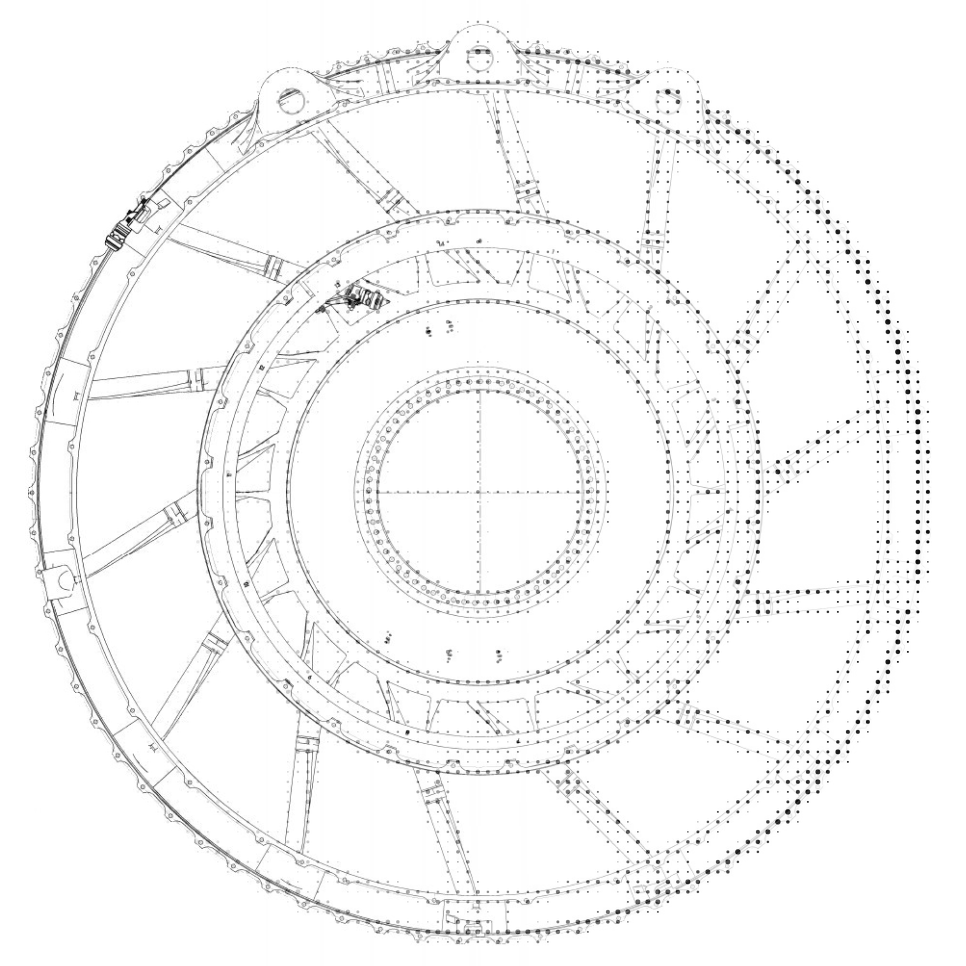
\includegraphics[width=0.51\textwidth]{fig/TRF Points 2.png}}
%% #2 Project partners:
{Håvard Norum GKN Aerospace}
%% #3 Summary:
{%
Analysis of geometric point cloud measurements pose very difficult challenges if removed from prior knowledge regarding the measurement process or measured object. The goal is to investigate how collections of 3D coordinates produced from 3D scan measurement systems can be structured, evaluated and analyzed solely from the information available in the data. The key difficulty is to create frameworks and methods able to be generally applicable to any unstructured point cloud.

The problems and dependencies regarding handling of unstructured geometric point clouds are presented alongside methods to resolve them. A method for utilizing the commercially available software ATOS Professional used by the aerospace manufacturer GKN Aerospace to find material thickness of welding junctions is discussed. A general method for determining material thickness for 3D scanned data with low curvature is proposed and implemented through Python programming.

The methods are continuously tested throughout the implementation of the presented material thickness method using fabricated 2D and 3D geometrical point cloud shapes with random noise to mimic real measurement variance. Large grounds for further work has been uncovered where parts of the presented methods have room for improvement as well as the discovery of other solutions and analytical methods.

}
\chapter{}
\chapter*{Preface}
\label{ch:preface}
\addcontentsline{toc}{chapter}{Preface}


% Må legge inn forklaring av størrelse/mengde i rapporten

This master's thesis is written as the individual finale of the Industrial Master study programme of Industrial IT and Automation at the Faculty of Technology, Natural Sciences and Maritime Sciences at the University of South-Eastern Norway, Porsgrunn. The work follows the requirement of the \textit{FMH606 Master's Thesis} subject and is a continuation of the work presented in the preliminary \textit{FM4017 Project} subject. It is throughout the thesis assumed that details about the TRF manufacturing process alongside it's hardware and software components are known from the previous work in \textit{Adaptive Welding Automation} (AWA) by Austefjord, R. 2020 \cite{Adaptive-Welding-Automation} and have thus not been explained twice.

The intent throughout the thesis is to infer useful insight and knowledge from information available within 3D point cloud datasets by utilizing studies on structuring, clustering and classifying algorithms. Ultimately presenting frameworks and methods for general solutions. The thesis has had a focus on method development and implementation, resulting in an equal priority on documenting the textual thesis as well as developing good code.

I would like to extend my gratitude towards my supervisors, \textit{Håkon Viumdal}, \textit{Ola Marius Lysaker} and \textit{Håvard Norum} for their professional expertise, guidance and feedback aiding me through the presented work. I also owe much to the coworkers at GKN that have enthusiastically included and involved me to work on equal footing throughout the three years spanning the IM Master's study. Finally I would like to thank my family and friends for the unconditional support and guidance making the years studying as enjoyable as they have been. 


The cover image is a reference to the GKN Aerospace produced TRF that initially sparked the interest for finding methods and ways to determine material thickness in new means. The style is a reference to the shifting focus of the real part to it's digital representation as a point cloud, the image is further discussed in (\ref{sc:Cover Image}).

\bigskip

Porsgrunn, \today.

\myauthor %% for thesis
%\myparticipants %% for project
%% table of contents
\tableofcontents
\addcontentsline{toc}{chapter}{\contentsname}

\listoffigures  % out-comment if unwanted

\addcontentsline{toc}{section}{\listfigurename}

%\listoftables  % out-comment if unwanted
%\addcontentsline{toc}{section}{\listtablename}

\chapter*{Nomenclature}
\label{sec:nomenclature}
List of abbreviations and symbols used throughout the thesis.

The \textit{italic} font style is used to emphasise important phrases and names.


\begin{longtable}{ll}
  \textbf{Symbol}    & \textbf{Explanation}\endhead         \\
    AWA              & Adaptive Welding Automation          \\
    CAD              & Computer-Aided Design                \\
    LIDAR            & Laser Imaging, Detection And Ranging \\
    ML               & Machine Learning                     \\
    PCA              & Principle Component Analysis         \\
    SAR              & Synthetic Aperture Radar             \\
    SLS              & Structured Light Sensor              \\
    STL              & Standard Triangle Language           \\
    SVD              & Singular Value Decomposition         \\
    TRF              & Turbine Rear Frame                   \\
    \(\lambda_{1D}\) & Linear Dimensionality                \\
    \(\lambda_{2D}\) & Planar Dimensionality                \\

\end{longtable}

\chapter{Introduction}
\label{ch:intro}

3D scanning has in recent years become more and more prevalent as the means to measure and digitize objects, surfaces and scenes in both scientific and commercial related applications. The reduction in both price and size alongside a gradual increase in accuracy of the measurement systems has made them widely available and applicable to a vast amount of use-cases. Typical examples are terrain and ground surveys by \textit{Laser Imaging, Detection, and Ranging} (LIDAR) or \textit{Synthetic Aperture Radar} (SAR). Which recently has taken the step from stationary ground surveys to aerial surveys with airplanes, drones and satellites providing data for previously untouched or unreachable terrain. Similar examples are 3D modelling for digital assets used in cinematics, videos or games. Where instead of building 3D assets from scratch, real objects are scanned and imported directly. Another example is it's use in archaeological surveys where excavation is either harmful or unfeasible.

At the manufacturing site GKN Aerospace Norway (GAN) this technology is currently used in production of aerospace engine components. As introduced in the previous master's project study AWA by Austefjord, R. 2020  \cite{Adaptive-Welding-Automation}, the key difficulties of manufacturing a Turbine Rear Frame (TRF) lay within the welding of forged and cold pressed metal-alloy components of varying thickness. For visual reference this is the part depicted on the front page of the thesis. To solve the key difficulties an automatized method of determining the material thickness in the welding junctions had to be developed. The suggested solution was presented as a system architecture containing three main steps. Firstly the raw material components were digitized through an optical 3D scanner where the resulting 3D point mesh was evaluated against an ideal CAD model to determine the material thickness at any point. Next the data was partitioned to only relate information regarding the welding junctions and transferred to a database for storage and accessibility. Lastly the data was accessed from the database and used to adjust the manufacturing parameters of the welding robot.

From the results of the master's project study it was concluded that the presented system architecture lacked the initial material thickness information from the ATOS Professional due to an outdated script. Upon further investigation and changes in GAN's production scheme it was decided that the master's thesis should continue the study of 3D scanned objects of similar nature the TRF. With a goal of achieving general material thickness evaluation either through the ATOS Professional software or directly from the point clouds produced by 3D measurement systems. 

Throughout this master's thesis problems and solutions regarding 3D scanned objects will be discussed. Straying from the highly implementation based master's project, the goal is now to present a more generalized theoretical study of the the 3D scanned objects.


\section{3D Scan as a Measurement System}
\label{sc:3d scan}
As 3D scanning units and modules has reached satisfactory levels of accuracy, price and size, they have gradually been introduced as measurement units replacing traditional methods. An example of this is how traditional "ground scaling" in large has been replaced by physical on site LIDAR or aerial LIDAR and SAR. The reasoning behind the transition is largely due to the reduction in measurement time and cost as well as the ease of access in certain use-cases. Being only restricted by the measurement systems field of view, 3D scanning offers superior usability when its accuracy is sufficient for the task.

3D measurements are mainly achieved through two basic principles, reflection timing or observational analysis. Methods such as LIDAR and SAR determine the distance by timing the return of their respective emitted wave signals. While other methods such as \textit{Structured Light Sensor} (SLS) and \textit{Photogrammetry} work by analyzing the observed "images" captured by specialised cameras. Similar for both methods are that they produce datasets containing the best approximations of distances that have been observed as a collection of points referenced by their distance in 3D space to the measurement system.

Today the most notable ways of representing these datasets are through \textit{Image-}, \textit{Volumetric-}, \textit{Mesh-} or \textit{Point cloud-} representations. This data describes the structure and geometry of the scanned objects, surfaces or scenes. Depending on the use-case the different forms of representations may have different merits, ranging from visualization to analysis. A handy visual guide for the different representations using the \textit{Stanford Bunny} \cite{Stanford-bunny} as render object can be seen in Figure \ref{fig:Common Representations of 3D data}.

\begin{figure}[H]
    \centering
    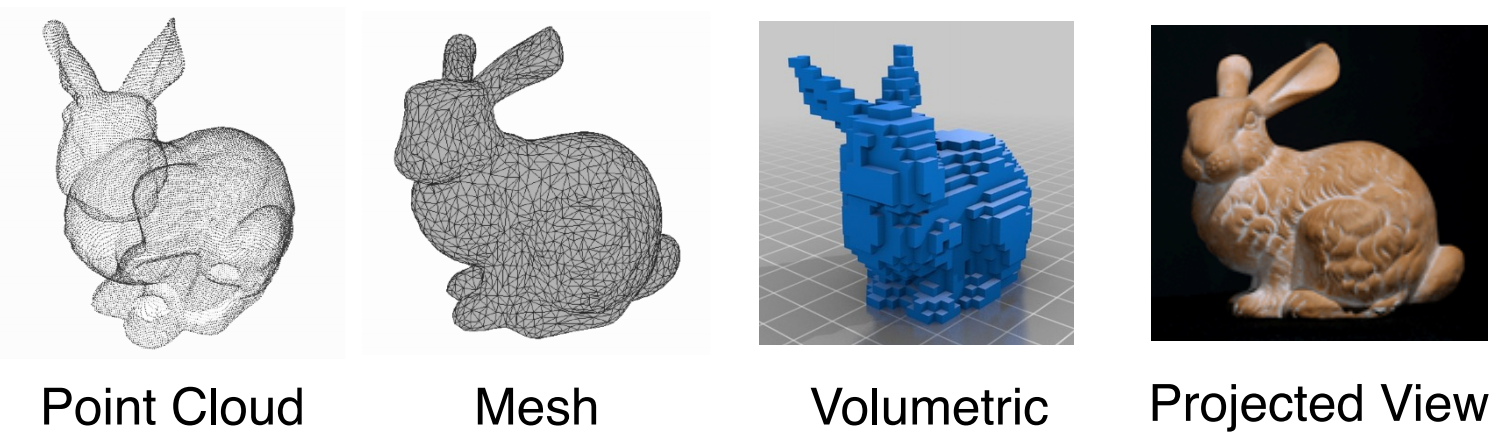
\includegraphics[width=0.99\textwidth]{fig/Stanford Bunny Point net.png}
    \caption{Common Representations Of 3D Data, Image In Courtesy Of Qi, C.R. et al., 2017 \cite{Point-net-presentation}.}
    \label{fig:Common Representations of 3D data}
\end{figure}
\clearpage
\subsection{Image or Projected View Representation of 3D Data}
\label{ssc:image}
The Image-based or "2D" representation of a 3D object is achieved through capturing images of the object at different view-points as demonstrated in Figure \ref{fig:2D representation of 3D}. This is particularly beneficial due to the vast amount of work that has been done surrounding analysis of 2D images. Notably methods such as image feature recognition, edge detection, classification and colour scheme analysis may be used directly in tandem with this form of representation.

\begin{figure}[H]
    \centering
    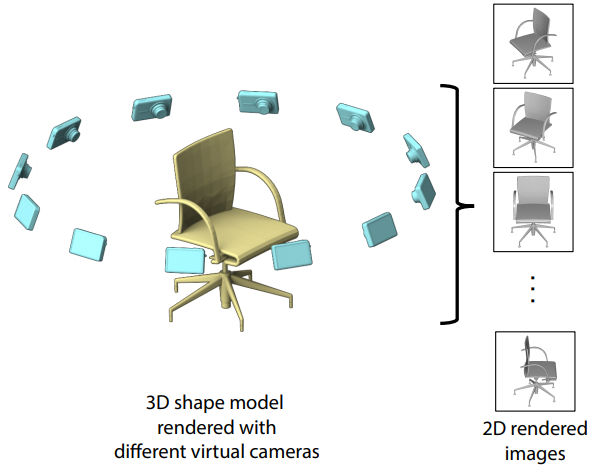
\includegraphics[width=0.42\textwidth]{fig/3D to 2D.png}
    \caption{2D Representation Of 3D Object, Image In Courtesy Of  Su, H. et al., 2015 \cite{2D-3D}.}
    \label{fig:2D representation of 3D}
\end{figure}

This representation however lacks the true "3D" aspect required for other methods of analysis such as volume, density, depth and other features that requires more than two dimensions. Notably there has been done work on reconstructing 3D objects from 2D images, Su, H. et al., 2015 \cite{2D-3D} and also neural networks capable of mapping depth in images, Zhou, T. et al., 2017 \cite{Depth}. This may in the future make the image representation very valuable for both 2D and 3D analysis.

This representation is currently best suited for simple 2D visualisation and in depth 2D analysis.
\clearpage
\subsection{Volumetric Representation of 3D Data}
\label{ssc:volumetric}
The volumetric representation of a 3D object describes the dataset in voxels otherwise referred to as "3D pixels". These are size variable cubes defined by a length, height and depth together with information regarding their connected neighbours. They are most commonly used in medical environments to determine volumes and provide quick 3D visualization. An example of this representation is provided in Figure \ref{fig:Volumetric representation of 3D}. This representation is best suited for quick 3D visualization and simple 3D analysis.

\begin{figure}[H]
    \centering
    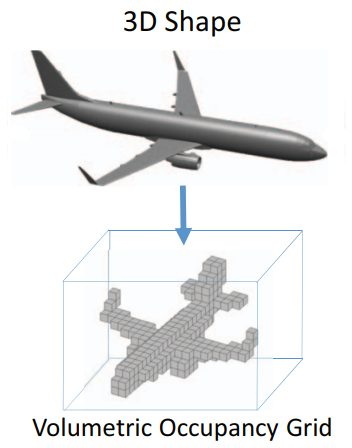
\includegraphics[width=0.38\textwidth]{fig/3D Volumetric.png}
    \caption{Volumetric Representation Of 3D Object, Image In courtesy Of  Qi, C. R. et al., 2016 \cite{3D-Volumetric}.}
    \label{fig:Volumetric representation of 3D}
\end{figure}


\subsection{Mesh Representation of 3D Data}
\label{ssc:meshes}
The surface-based mesh representation of 3D objects describe the triangulated external perimeter of the scanned object. Often produced from point clouds, this representation contains both information regarding the coordinates of the points as well as which other points make up the perimeter-triangles connected to that point. Displayed in Figure \ref{fig:Stanford Bunny Mesh} meshes attempt to optimize the grid such that it is fully connected and closed. This can be further scaled up and down which means that there exist cases where the mesh has to interpolate across "incomplete data". Similarly holes or missing data has to be enclosed such that the mesh often is extrapolated beyond the original dataset in order to ensure a fully connected and closed surface.

\begin{figure}[H]
    \centering
    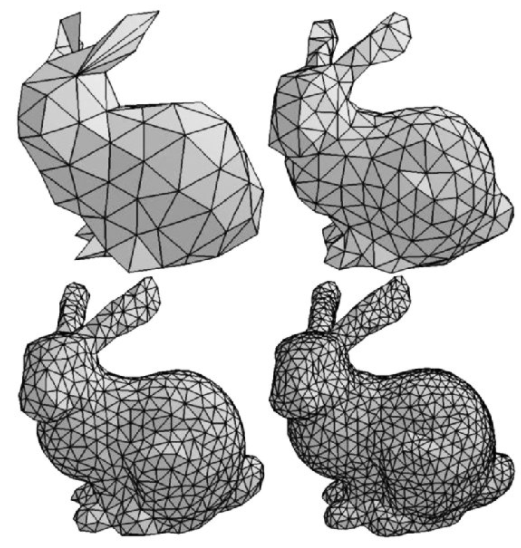
\includegraphics[width=0.35\textwidth]{fig/Stanford Bunny Mesh.png}
    \caption{Mesh Representation Of The Stanford Bunny \cite{Stanford-bunny} In Courtesy Of Novaković P.}
    \label{fig:Stanford Bunny Mesh}
\end{figure}

This representation has close ties to graphs and is very well suited for creating digital aspects or replications of physical objects. It provides good visualization and possibilities for in depth 3D analysis.

\subsection{Point Cloud Representation of 3D Data}
\label{ssc:point clouds}
The Point-based representation of 3D objects describe the 3D coordinates of all measured points in a dataset. Commonly referred to as a Point cloud, the representation can be considered as the unedited raw output of a 3D scan as displayed in Figure \ref{fig:Stanford Bunny Point Cloud}. Depending on the accuracy and limits of the measurement system, a point cloud may be highly varied in regards to point density. Together with the coordinates, the point can have descriptors such as color and temperature if such data also is available. 

\begin{figure}[H]
    \centering
    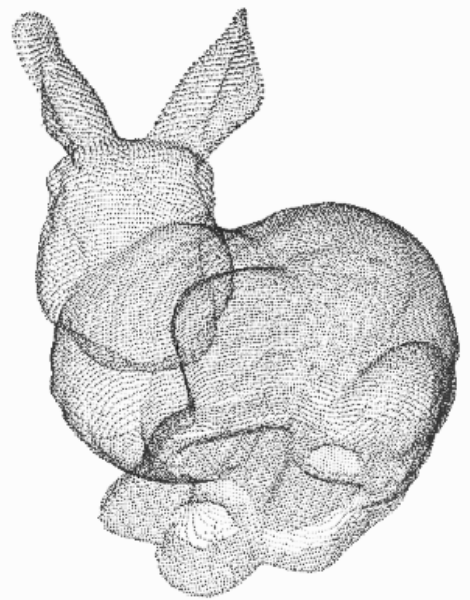
\includegraphics[width=0.25\textwidth]{fig/Stanford Bunny Point Cloud.png}
    \caption{Point Cloud Representation Of The Stanford Bunny \cite{Stanford-bunny} In Courtesy Of Qi, C. R. et al., 2017  \cite{Point-net-presentation}.}
    \label{fig:Stanford Bunny Point Cloud}
\end{figure}


This representation is best suited for in depth 3D analysis without compromising any information.

For the work in this master's thesis the methods will be developed from the point cloud representation as it most closely resembles the general raw data-output of any 3D scanning system and retains the maximum amount of information.

\section{Problem Description}
\label{sc:Problem Description}
The intent of this section is to introduce the problems surrounding developing \textit{General Point Cloud Methods}, \textit{General Material Thickness Evaluation} and of \textit{Scripting the ATOS Professional Software}.

\subsection{General Point Cloud Methods}
\label{sub:General Point Cloud Methods}
Datasets produced by the means of 3D scanning varies almost indefinitely from object to object. Moving, rotating, altering or exchanging the scanned object will result in a completely unique dataset. Measurement uncertainties, accuracy and resolution also ensures that any two scans would be unique though similar. Temperatures, pollutants, obstructions, air currents and all other conceivable sources of noise likewise has altering effects on the final dataset. Much of this variability bears little significance because it often contributes orders of magnitude less to the total deviation from the theoretical ideal when compared to the accuracy of the measurement system.

Out of the sources of variability there are mainly three that pose a challenge when attempting to generalize methods across a large manifold of datasets. The first of which is the \textit{point density} in the dataset. Example illustration shown in Figure \ref{fig:Point density on randomly distributed disks.}.

\begin{figure}[H]
  \centering
  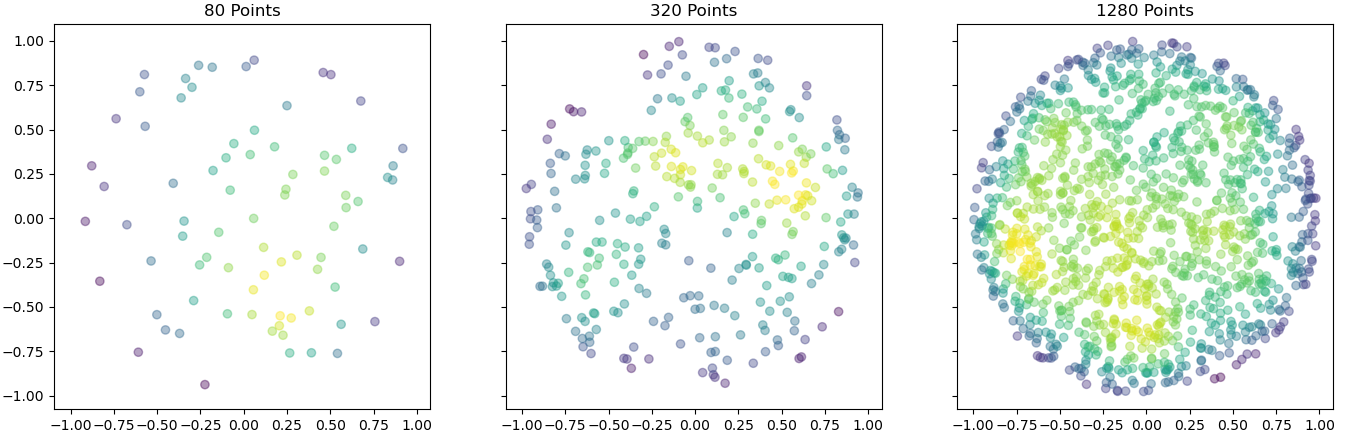
\includegraphics[width=0.99\textwidth]{fig/80_320_1280 points.png}
  \caption{Heat Mapped Point Density Distribution On Disks For Random Points.}
  \label{fig:Point density on randomly distributed disks.}
\end{figure}

Measuring a perfectly flat and rectangular 2D surface (plane) with a flawless measurement system, the surface could in theory be represented by the four edges of the plane. Such a scan would produce a dataset of only four points while perfectly representing the real object. Reintroducing the notion that the surface might not be perfectly flat and that there certainly are measurement variances and uncertainties that compound across the surface. The dataset would include far more points to represent the scanned object. This can be further complicated by scanning a more complex surface such as a sphere. Considering a perfect sphere, the ideal point cloud representation would be infinitely dense as there would be no edges in the object that could simplify the representation. Comparing the two ideal representations there is both a limit to how sparse and dense the point density can be within a dataset. Where it is practically impossible to reach either end of the ideals for a real measurement system. The resulting point density in the dataset is then tightly connected to the capabilities of the measurement system and the type/shape of object scanned. Resulting in an inherently infinite variance in datasets depending on what is being measured and what measured them. This means that methods applied to such datasets have to be invariant to point density, e.g. if the goal is to classify a plane, it should be able to classify the plane regardless of the dataset consists of four points or one million.

\bigskip
Another challenge when working with point clouds is the topic of \textit{orientation}. The notion of up/down, left/right, front/back does not simply apply to objects that have been 3D-scanned. The objects can be placed in any position/orientation within the measurement systems viewpoint. Likewise, the measurement system can be placed in any position/orientation surrounding the object. This fact decouples any notion of orientation in the dataset and imposes the frame of reference from the measurement system to the measured object. Resulting in any point within the dataset soley being a coordinate point based on the measured distance from the measurement system. This means that methods applied to such datasets have to be invariant to orientation and reference systems, e.g. "Up" can't simply be defined as increasing "z" values.

\bigskip
Another general challenge is that a dataset does not posses any prior heuristic or empirical knowledge regarding itself as the only information available in such a dataset is the individual coordinates of the points. Importantly this means that any single point has no information regarding its neighbouring points or if that point is part of feature "\textit{X} or \textit{Y}". At first glance the lack of this knowledge within a dataset might not be thought of as
particularly important. A given object does after all not need to  know what or where it is in order to exist.
Which is to say that for the object, only it's information is important, not the knowledge.\clearpage

\begin{figure}[H]
  \centering
  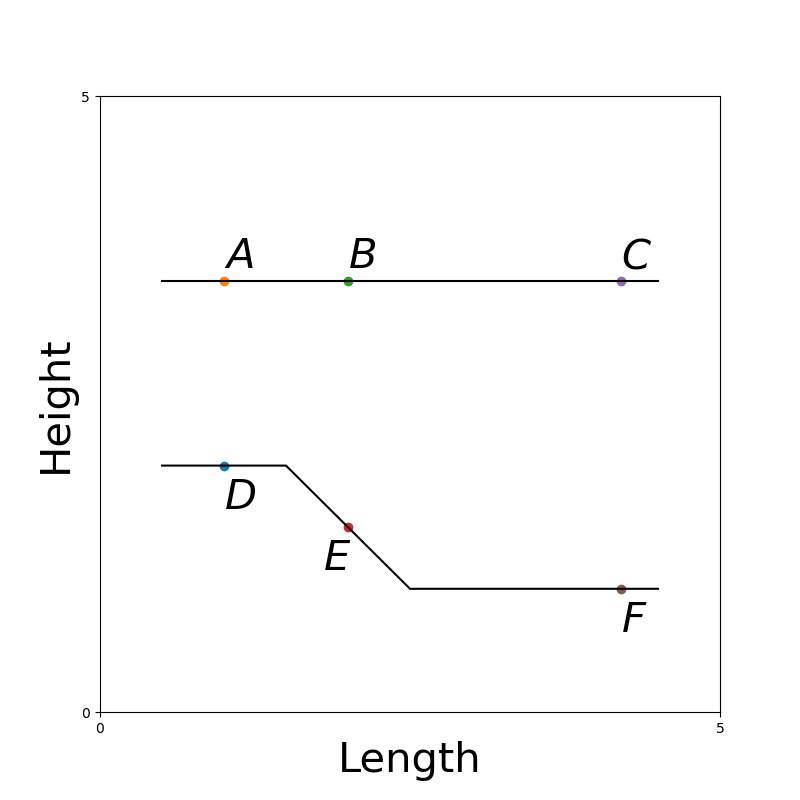
\includegraphics[width=0.325\textwidth]{fig/Cross1.png}
  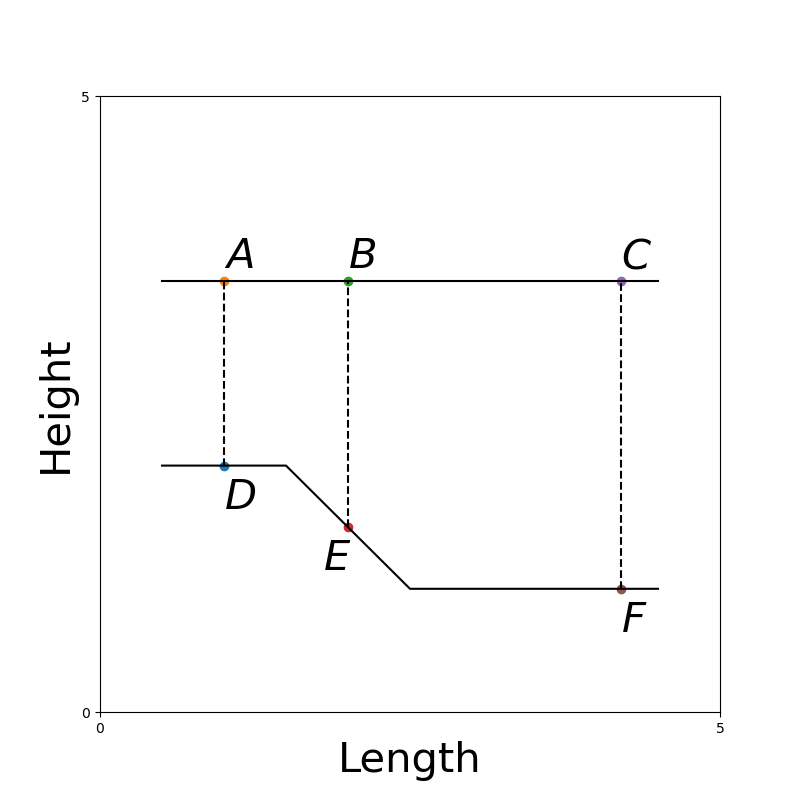
\includegraphics[width=0.325\textwidth]{fig/Cross2.png}
  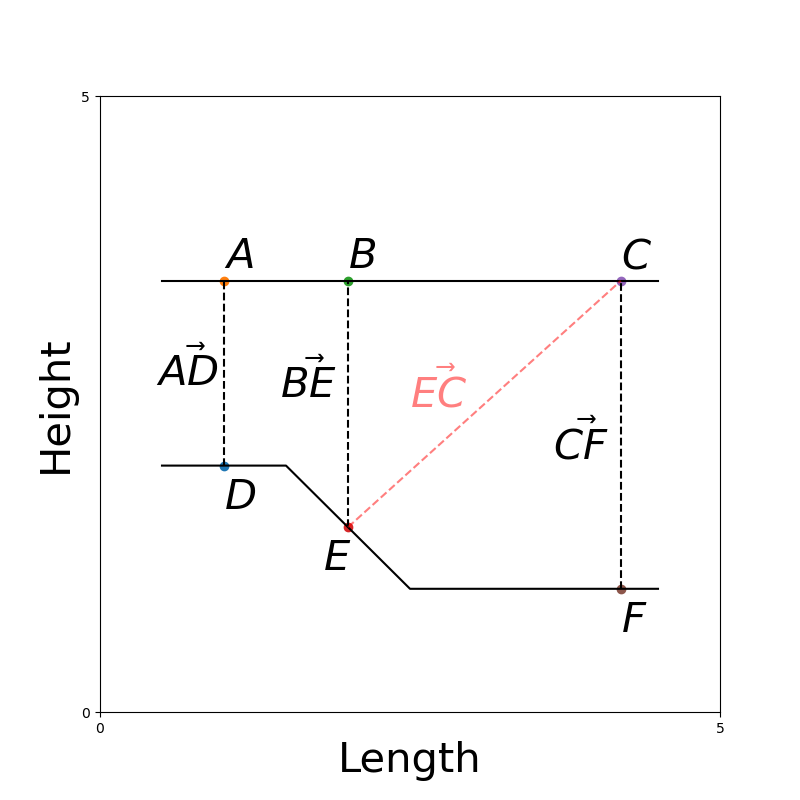
\includegraphics[width=0.325\textwidth]{fig/Cross3.png}
  \caption{2D Material Thickness Example Plate With Point-wise Material Thickness Pairing.}
  \label{fig:Metal Plate Cross-section}
\end{figure}

To illustrate these three general challenges with one example, Figure  \ref{fig:Metal Plate Cross-section} depicts a 2D cross section of a metal plate. The top surface is defined by the 3 points (\textit{A, B} and \textit{C}) which is distributed linearly along the length of the plate. The bottom surface is comprised of the points (\textit{D, E} and \textit{F}) where the height of the surface varies along the length of the plate. The goal is to find the material thickness, defined in this case as the distance between the top and bottom surface in the height direction. In the way that this example is constructed, finding the material thickness is not very difficult. The solution is simply to calculate the \textit{Euclidean Distance} between the point pairs (\textit{A, D}), (\textit{B, E}) and (\textit{C, F}). However, consider a change in \textit{point density}, let the bottom surface now be defined by 9 points along the surface. Point pairs can no longer be formed directly in the vertical height direction for every point, which means that some sub-optimal point pairing has to be made for at least 6 of the points on the bottom surface. Here the same calculation would not result in the correct material thickness, take Figure \ref{fig:Metal Plate Cross-section} vector \( \vec{EC}\) as an example. The next, maybe obvious problem is that if the plate was rotated even slightly, e.g. it's \textit{orientation} changed, the height direction would no longer equate to the material thickness. Similarly if the shape changed from a plate to a curved object, the material thickness might not even be defined in the same direction across the entire surface. Lastly, none of the points inhabit some \textit{knowledge} regarding whether it is located on the top or bottom surface. Nor any information regarding what point it is supposed to be paired with in order to calculate the distance.

From these challenges it can be deduced that general methods has to be invariant to variations in point density, orientations, shapes and heuristic and empirical knowledge.\clearpage

\subsection{General Material Thickness Evaluation}
\label{sub:Material Thickness}
Material thickness can generally be thought of as the distance between two opposing sides of the same fully-connected surface. For simple shapes such as cubes this usually is the shortest of the three dimensions with regards to height, width and length. The material thickness can then be defined by that direction across the entire object. However for more complex shapes with curvatures, holes and extrusions, the material thickness can't be defined solely in one direction as the material thickness now depends directly on the point of measurement. Material thickness should then be defined as the distance from the point of measurement to the opposing side of the same fully-connected surface. Or in general as the shortest distance to another opposing surface.

From a measurement standpoint, material thickness is a relatively simple property to measure as long as the direction of the measurement is defined. This definition is however often made from prior experience or knowledge. The problem in defining the direction is often to \textit{know} where one surface ends and the next begins, while also \textit{understanding} that one surface opposes the other in a "back/front", "top/bottom" or "left/right" pairing. 

Proposing a method that may be generally applicable thus has to rely on the same prior knowledge or be able to incite it by itself. There is some return of value presented by the increase in accuracy from material thickness measurements being done on a costly but accurate 3D scan apposed to a manual measurement. However the greatest return would be if the measurement could be achieved autonomously without relying on any prior knowledge or experience.

\subsection{Scripting ATOS Professional Software}
\label{sub:Scripting ATOS Professional Software}
To summarize the problem description regarding the scripting of the ATOS Professional software from Austefjord, R. 2020 \cite{Adaptive-Welding-Automation} we have:

A script capable of autonomously detecting and evaluating the material thickness within the welding junctions has to be developed. Using built-in functions of the software such as script-ability and material thickness evaluation compared to CAD files.


\chapter{Methods}
\label{ch:Methods}

In this chapter methods for generalizing and classifying the 3D point cloud datasets are presented through the subsection \textit{General Evaluation Framework}. Followed by methods for evaluating material thickness in \textit{Material Thickness} and resolving the method for scripting \textit{ATOS Professional}.


\section{General Evaluation Framework}
\label{sec:General Evaluation Framework}
To tackle the unending quarrel of density variance, lack of orientation and knowledge, some known theory and mathematical theorems can be considered in order to form a basic "reference" frame for the unstructured 3D point cloud measurements. Making it possible for more sophisticated, general and specific methods to be applied to the datasets without having to rely on specialised heuristic or empirical knowledge.

The intent and goal for this section is to introduce the methods that extrapolate upon the information available in the datasets. 

\subsection{Graph Theory as a Framework}
\label{sub:Graph Theory}
\begin{wrapfigure}{r}{0.35\textwidth}
    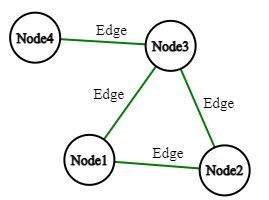
\includegraphics[width=0.9\linewidth]{fig/Node Edge.png}
    \caption{Structure Of Nodes And Edges In Graphs.}
    \label{fig:Nodes and Edges}
\end{wrapfigure}
When the data is presented in the form of either \textit{volumetric}, \textit{point cloud} or \textit{mesh} structures, it is simple to formulate many of the questions as graph theory problems. In graph theory the data is generally presented in terms of nodes and edges as shown in Figure \ref{fig:Nodes and Edges}. For \textit{volumetric} representation the voxels would represent the nodes while the connections to the nearby voxels define their edges. In a point cloud the points directly correspond to nodes whereas the edges are the distances to all other points. A mesh structure is inertly already a graph and thus require no new formulation. Common for all of these representations is that the graphs are undirected, meaning there is no preferred direction to the edges.


There exist a couple ways to represent graphs, most commonly they are represented through either an adjacency matrix, ref. Figure \ref{fig:Adjacency Matrix} or an adjacency list, ref. Figure \ref{fig:Adjacency List}. Considering that an adjacency matrix lists all possible edges between nodes even if there are none, the size of the matrix grows proportionally with the size of the dataset squared. An adjacency list however only denotes which edges exist and thus only grows proportionally with the amount of connections/edges in the dataset. Datasets produced from 3D scanning will be very large thus it only makes sense to continue with the representation in form of an adjacency list.

\begin{figure}[H]
  \centering
  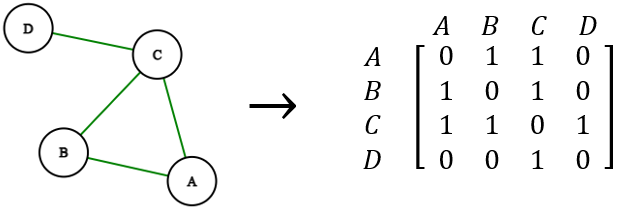
\includegraphics[width=0.5\textwidth]{fig/Adjecency Matrix.png}
  \caption{4-Node Graph And It's Corresponding Adjacency Matrix.}
  \label{fig:Adjacency Matrix}
\end{figure}
\begin{figure}[H]
  \centering
  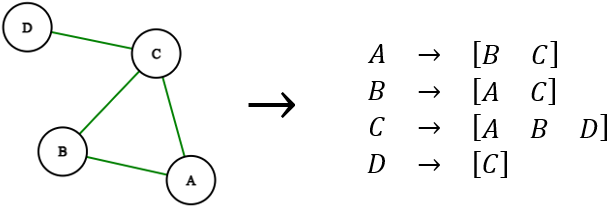
\includegraphics[width=0.5\textwidth]{fig/Adjecency List.png}
  \caption{4-Node Graph And It's Corresponding Adjacency List.}
  \label{fig:Adjacency List}
\end{figure}


Depending on the format of the input, the adjacency lists may be either sparse or dense depending on the amount of edges coupled to a given node. For both the \textit{volumetric} and \textit{mesh} representation, there only exist a handful of edges per node, making them naturally sparse. This is great for low memory consumption and computational power. Point clouds are however naturally dense since all nodes are connected to each other, effectively making the representation an adjacency matrix filled with ones. Working with point clouds as graphs is therefore cumbersome if computational power and memory is limited. Luckily most of the edges are abundant and provide no particularly insightful information. The adjacency list may therefore be shorted to only contain a certain specified number \(k\) edges of interest.
\clearpage
\subsubsection{KD-Trees}
\label{subsub:KD-Trees}
As is the case with both the \textit{volumetric} and \textit{mesh} representations, the general interest in \textit{point clouds} are the closest neighbours of the points/nodes. Evaluating the \(k\) nearest neighbours of a graph is fortunately a widely covered problem with many solutions. One of which is the "K-Nearest-Neighbour" (KNN) search introduced by Friedman, J. H. et al., 1977 \cite{kd-tree}. This function works by structuring the data in a binary tree known as a kd-tree. This structure separates the dataset based upon a defined delimiter which in this case has the goal of grouping similar data. From Friedman, J. H. et al., 1977 \cite{kd-tree} the tree delimiter is the point in the dataset where the greatest spread occurs, e.g. the difference between the minimum and maximum values. This equates to be the median of the dataset and is known as the \textit{Standard Split}. The delimiter used for constructing the kd-trees has further been improved through several iterations where today the most commonly applied is the \textit{Canonical Sliding-Midpoint Split} introduced by Maneewongvatana, S. et al., 1999 \cite{kd-tree-sliding-midpoint}. Once a kd-tree is constructed, any point \(n\) can be queried for their nearest \(k\) neighbours without having to calculate the distances to all possible points in the dataset. This is made possible by only evaluating the points in the same tree cluster/branch, greatly reducing the computational effort.

Using this method, point clouds can be formulated as graphs without sacrificing memory or computation power and can be represented by an adjacency list equal to the ones used for both \textit{volumetric} and \textit{mesh} structures.

\subsection{Neighbourhood Parameterization}
\label{sub:Neighbourhood Parameterization}
For the sake of analyzing the dataset, there is often a desire to find similarities or features within the data in order to classify points or areas depending on the grouping. Such data clusters can be evaluated with different tools, ranging from shape recognition (Barr, A. H., 1981 \cite{Superquadrics}) to modern day neural network classifiers (Zhu L. et al., 2019 \cite{nn-point-cloud-classifier}).
Direct examples are separating the bare ground from vegetation (Jiang, Y. et al., 2019 \cite{nn-crops}) and from urban features (Weinmann, M. et al., 2015 \cite{optimalNeighbourhood}). The list of possible applications are not short, indicating that finding such data clusters within the point cloud could provide highly insightful and valuable information. 

There are several methods for finding such clusters, however many of them are very specialised towards which objects, surfaces or scenes that are expected as inputs, or from which measurement system the data was collected. The problem is in general that if given an ordinary coffee-mug, two different measurement systems could provide vastly different point resolutions of the mug once scanned. Say one is a point cloud of 30 000 points \(A\), while the other is 5 000 points \(B\). If an algorithm should classify clusters that are either flat or have a curvature above a certain percentage. The same algorithm might evaluate the scanned mug \(A\) to be flat in a region given by a point on the mug and the \(k=10\) closest points. Whereas for \(B\), due to the lower point density, the same ten closest points would be much further removed in distance, revealing that there was a curve. Even worse would be to use the same algorithm on an entirely different object. It is pretty obvious that the number of \(k\) nearby neighbours has to have some form of variability with the point density as well as the shape of the object, surface or scene.

In Weinmann, M. et al., 2014 \cite{optimal-K-Nearest-Neighborhood} it is said that the best selection of the number \(k\) nearest neighbours can be determined by selecting the value of \(k\) which yields the minimum \textit{Shannon Entropy}. This ensures that the point selection includes enough points that a local descriptive cluster can be formed while also ensuring that the greatest local information divide has been reached.

\subsubsection{Shannon Entropy for 3D Structures}
\label{subsub:Shannon Entropy}
Presented in \textit{A Mathematical Theory of Communication}  by Claude Elwood Shannon \cite{Shannon-Entropy}, the Shannon Entropy is used to evaluate the information entropy of a given probability distribution. Denoted by \(H(x)\) the Shannon Entropy is a measure of the uncertainty of an event \("x"\), ranging from \(0 \to \inf\). If the probability distribution only has one outcome, there exist no uncertainty in the distribution and the Shannon Entropy equates to \(0\). Mathematically the function is represented in (\ref{eq:Shannon Entropy})
\begin{equation}
    \label{eq:Shannon Entropy}
    H(x) = -\sum_x{{P(x)\log{P(x)}}}
\end{equation}
were \(P(x)\) is the probability distribution of events \("x"\) and \(\log\) is the base-2 logarithm. An unlikely outcome will score a high Shannon Entropy value, whereas the most likely outcome will score the lowest value of Shannon Entropy.

Considering a point \(p_0\) in the dataset and it's nearest \(k\) neighbours. A covariance matrix \(C\) can be calculated for the collection of points from \(p_0 \to p_k\) as shown in (\ref{eq:Mean}) and (\ref{eq:Covariance Matrix})
\begin{align}
\label{eq:Mean}
    \Bar{p} &= \frac{1}{1+k}\sum_{i=0}^k p_i \\
\label{eq:Covariance Matrix}
    C  &= \frac{1}{1+k}\sum_{i=0}^k (p_i-\Bar{p})(p_i-\Bar{p})^T
\end{align}
where from the covariance matrix, the three eigenvalues \(\lambda_1 \geq \lambda_2 \geq \lambda_3\) can be calculated. Such that \(\lambda_1\) explains the greatest variance in the point collection, followed by \(\lambda_2\) and \(\lambda_3\). Since the dimensionality of the dataset is 3D, 100\% of the variation can be explained by the three eigenvalues. Following  Weinmann, M. et al., 2014 \cite{optimal-K-Nearest-Neighborhood}, the eigenvalues can be normalized giving the eigenvalues \(e_1\), \(e_2\) and \(e_3\) as defined in (\ref{eq:e1}), (\ref{eq:e2}) and (\ref{eq:e3}) distributed from \(0 \to 1\) 
\begin{align}
\label{eq:e1}
e_1 &= \frac{|\lambda_1|}{|\lambda_1|+|\lambda_2|+|\lambda_3|}   \\
\label{eq:e2}
e_2 &= \frac{|\lambda_2|}{|\lambda_1|+|\lambda_2|+|\lambda_3|}    \\
\label{eq:e3}
e_3 &= \frac{|\lambda_3|}{|\lambda_1|+|\lambda_2|+|\lambda_3|}
\end{align}
where \(|\lambda_n|\) in this thesis is the abs(Re(\(\lambda_n)\)) of eigenvalue \(n\).\footnote{The \(|\lambda_n|\) operation is theoretically unnecessary since the covariance matrix \(C\) is said to be positive definite. This claim is beyond the scope of this thesis, however the interested reader is referred to Weinmann, M. et al., 2014 \cite{optimal-K-Nearest-Neighborhood} page 5.}
It is further shown in  Weinmann, M. et al., 2014 \cite{optimal-K-Nearest-Neighborhood} that the eigenvalues can be exploited to describe certain dimensionality features such as \textit{linearity} \(L_\lambda\), \textit{planarity} \(P_\lambda\)  and \textit{scattering} \(S_\lambda\) described in (\ref{eq:Linearity}), (\ref{eq:Planarity}) and (\ref{eq:Scattering})
\begin{align}
\label{eq:Linearity}
L_\lambda &=\frac{e_1-e_2}{e_1}  \\
\label{eq:Planarity}
P_\lambda &=\frac{e_2-e_3}{e_1}  \\
\label{eq:Scattering}
S_\lambda &=\frac{e_3}{e_1}    .
\end{align}
As the eigenvalues are normalized and range from \(0 \to 1\) and importantly sum up to one for both \(e_1 + e_2 + e_3 = 1\) and \(L_\lambda + P_\lambda + S_\lambda = 1\), the values can be thought of as "pseudo" probabilities. The value of \(e_1\) will for instance indicate the "probability" of the dataset being described solely by \(e_1\). Likewise the "probability" that the dataset is linear or one-dimensional can be evaluated by \(L_\lambda\). The values can then carefully be applied to the Shannon Entropy function, ensuring that no eigenvalue equates to 0 by adding an infinitesimally small \(\epsilon\). From this the \textit{eigenentropy} \(e_\lambda\) and \textit{Shannon Entropy} \(E_\lambda\) are defined according to (\ref{eq:Shannon Entropy}) as follows in (\ref{eq:eigenentropy}) and (\ref{eq:shannonentropy})
\begin{align}
\label{eq:eigenentropy}
e_\lambda &= - e_1\log e_1 - e_2\log e_2 - e_3\log e_3  \\
\label{eq:shannonentropy}
E_\lambda &= - L_\lambda\log L_\lambda - P_\lambda\log P_\lambda - S_\lambda\log S_\lambda .
\end{align}

\clearpage


\section{Material Thickness}
\label{sec:Material Thickness}
In this section the approach of creating a general applicable method for evaluating \textit{material thickness} is described. The methods are developed to match the underlying human intuition towards material thickness while gradually utilizing the general methods presented in \textit{General Evaluation Framework} (subsection \ref{sec:General Evaluation Framework}). The methods are presented in order from least to most general.

\subsection{Euclidean Distance}
\label{sub:Euclidean Distance}
Given the simple rectangular dataset in Figure \ref{fig:Sample Dataset} with respects to material thickness. Much alike the 2D example in \textit{General Point Cloud Methods} (subsection \ref{sub:General Point Cloud Methods}) this 3D dataset has points distributed such that the height direction can be defined as the direction of the material thickness. The points are also distributed evenly across a grid such that the direction-lines in the grid intersecting the points are \(\perp\) to each other.
\begin{figure}[H]
    \centering
    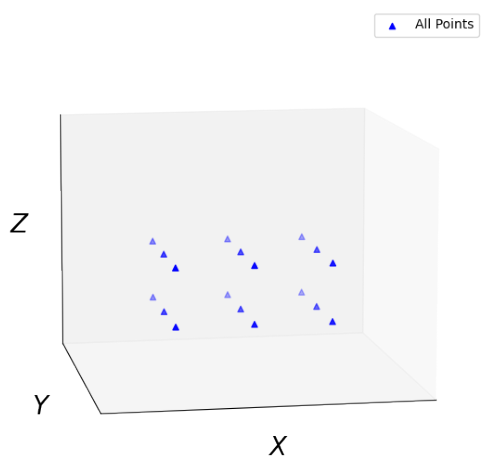
\includegraphics[width=0.45\textwidth]{fig/Sample Data-set.png}
    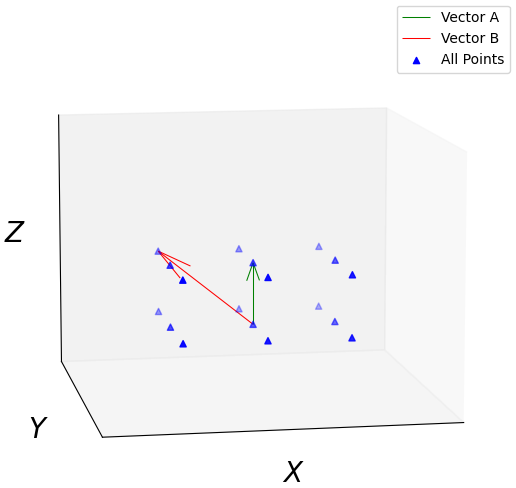
\includegraphics[width=0.45\textwidth]{fig/Sample Data-Set Random Points vectors.png}
    \caption{3D Sample Dataset With Two Distance Vectors.}
    \label{fig:Sample Dataset}
\end{figure}
The distance between any point pair $p$ and $q$ can be calculated as the \textit{Euclidean Distance} \("dist(p,q)"\) between them as seen in (\ref{eq:Euclidean Distance})
\begin{align}
    \label{eq:Euclidean Distance}
    dist(p,q) = \sqrt{(q_x-p_x)^2+(q_y-p_y)^2+(q_z-p_z)^2}.
\end{align}
Knowing that \("Z"\) is the direction of the material thickness \textit{Vector A} from Figure \ref{fig:Sample Dataset} equates to the correct point pairing to determine the material thickness.

This method is comparable to manual thickness measurements with e.g. calipers. The direction of the measurement is known and point \(p\) and \(q\) is selected to adhere to this knowledge. This makes the method not generally  applicable as it relies solely on heuristic and empirical knowledge. 


\subsection{Parallel 2D Planes}
\label{sub:Parellel 2D Planes}
Given a box, book or simply a sheet of paper, our perception of depth within an object allows us to determine the direction of the material thickness almost immediately. We identify the surfaces on the objects and choose the ones with the smallest distance between as the depth.
Consider the same simple rectangular dataset in Figure \ref{fig:Sample Data-set} with respects to material thickness.
Expressing our intuition of depth, we have that the distance between the two ideal and parallel planes equates to the material thickness.

\begin{figure}[H]
  \centering
  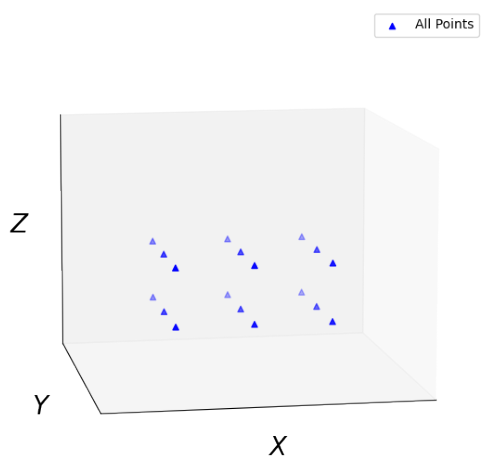
\includegraphics[width=0.45\textwidth]{fig/Sample Data-set.png}
  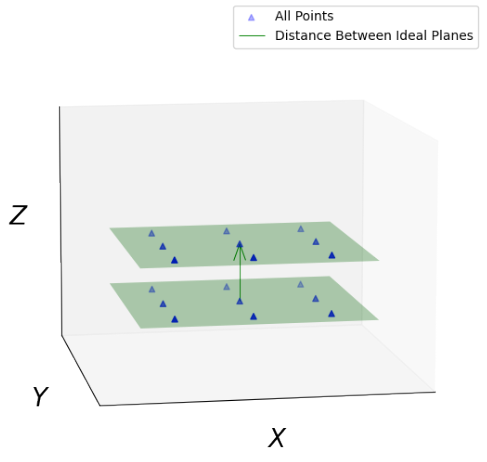
\includegraphics[width=0.45\textwidth]{fig/Sample Data-Set Ideal Planes.png}
  \caption{3D Sample Dataset With Two Ideal Planes Across The Bottom And Top Surface.}
  \label{fig:Sample Data-set}
\end{figure}

Expressing this mathematically the method can be divided into three steps: \(a)\), \(b)\) and \(c)\) each explaining the process taken to determine the material thickness. 

\(a)\) An initial point \(p_0\) has to be selected from where the material thickness should be evaluated. This may be done through the end-user's specific choice, a random selection or through an incremental loop if all points are to be evaluated. The only constraint is that the point \(p_0\) has to exist in the dataset.
\clearpage
\(b)\) A 2D plane has to be created through the point \(p_0\), such that the plane resembles the surface of the object. Generally this can be achieved with the function for a plane, described in (\ref{eq:Plane}) 
\begin{align}
    \label{eq:Plane}
    ax + by + cz + d &= 0 
\end{align}
where \((x, y, z)\) is a point located in the plane, while \([a, b, c]\) is a direction vector perpendicular to the plane. Having selected a point \(p_0\) in \(a)\), this only leaves the direction vector as unknown. Recalling that the direction of the material thickness is defined as the height or \("Z"\) direction in the dataset, the normal vector for the plane is known. Expressing the equation for a plane with respect to a point \(A=(x_0,y_0,z_0)\) and the plane's normal vector \(\vec{n}=[a,b,c]\) we have in (\ref{eq:Point Vector Plane})
\begin{align}
        \label{eq:Point Vector Plane}
    a(x-x_0) + b(y-y_0) + c(z-z_0) &= 0.
\end{align}


\(c)\) Steps \(a)\) and \(b)\) are repeated for a point on the opposing surface such that two parallel planes are formed. The material thickness can then be found from calculating the distance between the planes given by (\ref{eq:distacen between planes})


\begin{align}
\label{eq:distacen between planes}
dist &= \frac{|d_1-d_2|}{\sqrt{a^2+b^2+c^2}}. %\\
%\label{eq:distance between planes matrix form}
%d &= \begin{bmatrix} 
%    a_{11} & a_{12} & \vdots &\\
%    \vdots & \ddots & \vdots &\\
%    a_{K1} &        & \vdots &
%    \end{bmatrix}
\end{align}

This method more closely resembles our thought process when finding the material thickness of an object. Though relying on the prior knowledge regarding the direction of the material thickness. If the point pairing is selected at random, a distance will be found, however not necessarily in the direction of the material thickness as shown in Figure \ref{fig:Sample Data-set Evaluated at Random Points}.

\begin{figure}[H]
  \centering
  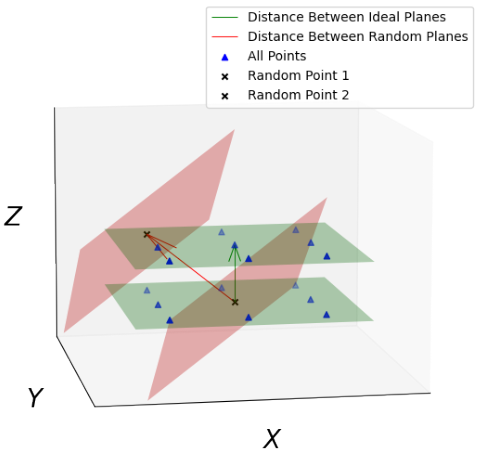
\includegraphics[width=0.45\textwidth]{fig/Sample Data-Set Random Points 1.png}
  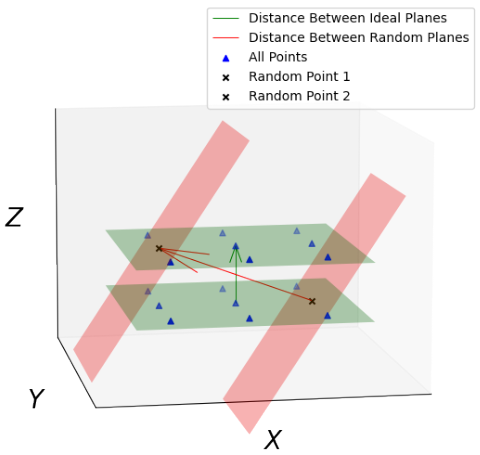
\includegraphics[width=0.45\textwidth]{fig/Sample Data-Set Random Points 2.png}
  \caption{3D Sample Dataset Where Material Thickness Is Evaluated At Random Points.}
  \label{fig:Sample Data-set Evaluated at Random Points}
\end{figure}

\subsection{Best-Fit Planes}

Evaluating the flaws of the \textit{Parallel Planes} method, the intention is not to find "a" plane, but a plane that represents the surface the selected point lies within. This can be achieved by evaluating the nearest neighbours of the initial selected point through a KD-tree search. In this way the closest \(k\) neighbouring points can be evaluated as a local cluster explaining the surface surrounding the initial point. From this cluster a 2D plane can be fitted to match the points through a least squares optimization problem. 
Implementing the least squares method in accordance with the matrix formulation described under the \textit{Ordinary Least Squares} page \cite{Ordinary-Least-Squares}. The cluster can be expressed as an overdetermined system on the form \(\sum_{j=1}^p X_{ij}\beta_j=y_i\text{, } (i=1,2,\dots,k)\text{, } (j=1,2,\dots,p) \) where \(p\) is the number of equation variables. Equation (\ref{eq:Plane}) can be solved for \textit{z} and expressed as \(y=X\beta\) where
\begin{equation}
    X = \begin{bmatrix} x_{1} & y_1 & 1 \\ x_{2} & y_2 & 1 \\ \vdots & \vdots & \vdots \\ x_k & y_k & 1 \end{bmatrix}, \text{ } \beta = \begin{bmatrix} a \\ b \\ d \end{bmatrix}     \text{ and }
    y = \begin{bmatrix} z_{1} \\ z_{2} \\ \vdots \\ z_k \end{bmatrix} \text{ for \(k\) points in the cluster.}
\end{equation}

A plane can then be fitted to match the points through a least squares optimization problem as formulated in (\ref{eq:Least Squares Planes}), (\ref{eq:Least Squares Planes Normal}) and (\ref{eq:Least Squares Planes Normal Best})
\begin{align}
    \label{eq:Least Squares Planes}
    \textit{arg min:  } S(\beta) &=\sum_{i=1}^n (y_i-\sum_{j=1}^p X_{ij}\beta_j)^2 =(y-X\beta)^2 \text{ where it follows that:} \\
    \label{eq:Least Squares Planes Normal}
    X^TX\beta & = X^Ty \\
    \label{eq:Least Squares Planes Normal Best}
    \beta &= (X^TX)^{-1}X^Ty \text{  .}
\end{align}

Demonstrated with 50 randomly distributed points in Figure \ref{fig:least squares}, this can be utilized in step \(b)\) from \textit{Parallel 2D Planes} (subsection \ref{sub:Parellel 2D Planes}) to form the plane representing the local surface.

\begin{figure}[H]
  \centering
  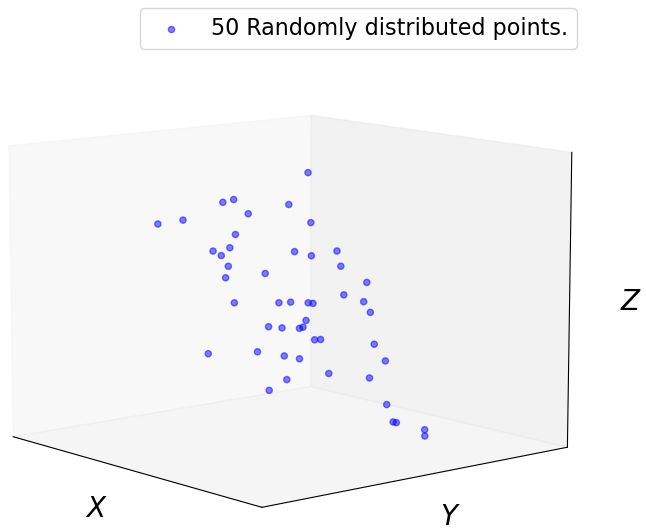
\includegraphics[width=0.41\textwidth]{fig/Plane 6.50.png}
  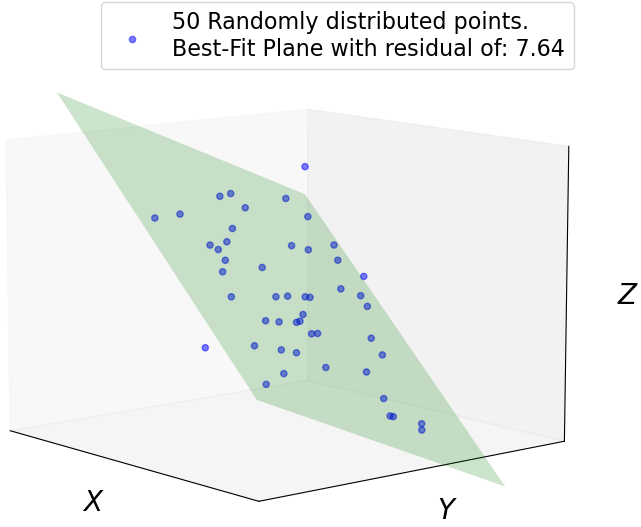
\includegraphics[width=0.41\textwidth]{fig/Plane 6.77.png}
  \caption{Example Of Least Squares Plane Fitting With 50 Randomly Distributed Points.}
  \label{fig:least squares}
\end{figure}

This improvement accomplishes an invariance to prior knowledge by removing the need to know the direction of the plane normal. However it is still very sensitive to both changes in point density and orientation as well as the initial selected point. This can be demonstrated in Figure \ref{fig:Sample Data-set with least squares} using the simple 3D dataset from (subsection \ref{eq:Euclidean Distance}).

\begin{figure}[H]
  \centering
  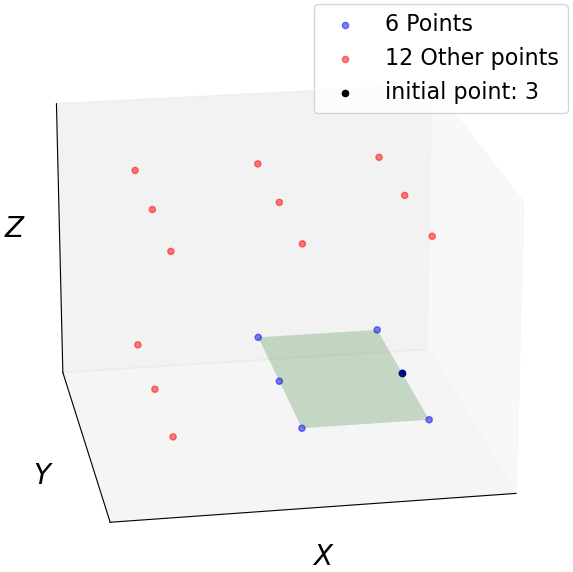
\includegraphics[width=0.32\textwidth]{fig/6 nearest points.png}
  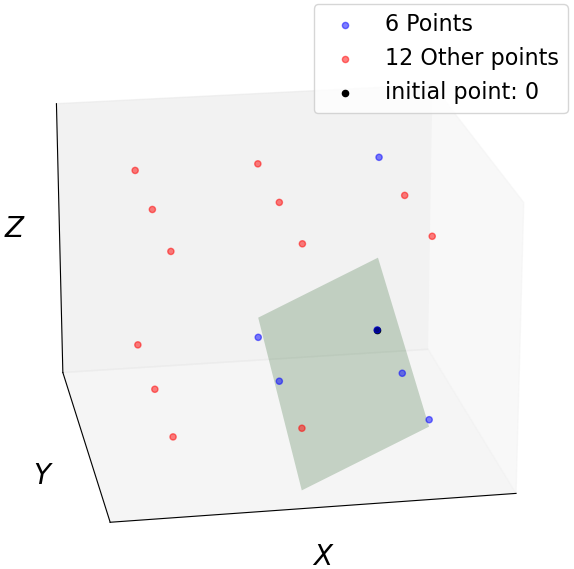
\includegraphics[width=0.32\textwidth]{fig/6 nearest points edge.png}
  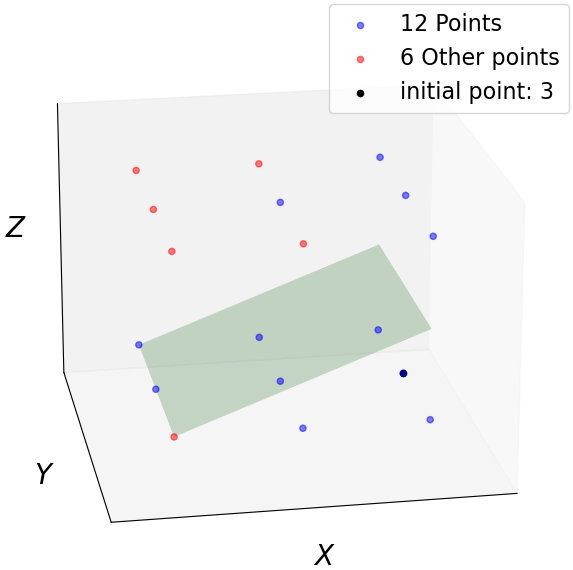
\includegraphics[width=0.32\textwidth]{fig/12 nearest points.png}
  \caption{Least Squares Plane Fitting On 3D Sample Dataset With Varying \(p_0\) And \(k\) Neighbouring Points.}
  \label{fig:Sample Data-set with least squares}
\end{figure}

Viewing Figure \ref{fig:Sample Data-set with least squares} from left to right, the different subplots showcase that 1) if the number of \(k\) nearest neighbours are properly selected (displayed as blue dots surrounding the black \(p_0\) initial point) a plane (displayed in green) can be created in the direction of the surface. 2) If the initial point lies such that one of the set number of closest neighbours lie on another surface, the plane is fitted across the two surfaces and fails to explain the singular surface of the initial point \(p_0\). Finally in 3) if the number \(k\) exceeds a certain threshold dependant on the point density, the plane will likewise fail to explain the surface surrounding the initial point as it is forced to include points in other surfaces.

There also exist a bias within the \textit{Least Squares} method used to fit a plane when it comes to the preferred direction to minimize the error. In this case the solution is solved for the \(z\) direction implying that for this dataset it is "known" that \(z\) or "height" is the preferred direction to optimize for.

\subsection{Neighbourhood Optimized Planes}
\label{sub:Neighbourhood optimized SVD Best-Fit Planes}
Once again reviewing the flaws of the previous method with respects to a general solution, there are mainly two improvements that can be implemented. Firstly the number of \(k\) nearest neighbours should be scalable depending on the surface where the initial point lies. For this the \textit{Shannon Entropy} (subsection \ref{subsub:Shannon Entropy}) can be incorporated to determine how many points should be evaluated before the "uncertainty" of the dimensionality in the cluster increases. In other words the Shannon Entropy should be minimized such that only points within a single plane should be included. The second improvement is to remove the bias towards any direction when fitting a plane to the cluster. This can be done through a \textit{Singular Value Decomposition} (SVD) such that the plane is fitted by allowing for errors across all the individual variables \(x\), \(y\), and \(z\), not restricting the error to only occur in one "known" vertical direction.

From \textit{Shannon Entropy for 3D Structures} (subsection \ref{subsub:Shannon Entropy}) we have that the dimensionality can be described by the normalized eigenvalues and eigenvectors. Notably a cluster of points can be said to confide within a 2D surface of arbitrary direction or rotation if the third eigenvalue is minimal. This can be explained by considering the normalized eigenvalues where \(e_1 \geq e_2 \geq e_3\) and \(e_1+e_2+e_3=1\). If the first eigenvalue \(e_1\) explains close to 100\% of the variation within the cluster, the points that make up the cluster would only lie along the first eigenvector or in other words along a linear line. If \(e_1 \text{ and } e_2\) explain 50\% of the variance each, the points that make up the cluster would be spread out symmetrically across the first and second eigenvector. These two concepts related to the eigenvalues are demonstrated in Figure \ref{fig:Linear system}.

\begin{figure}[H]
  \centering
  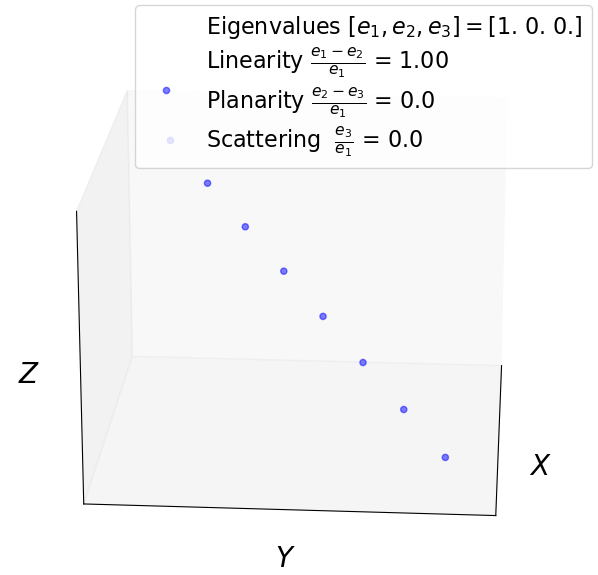
\includegraphics[width=0.48\textwidth]{fig/Linear System.png}
  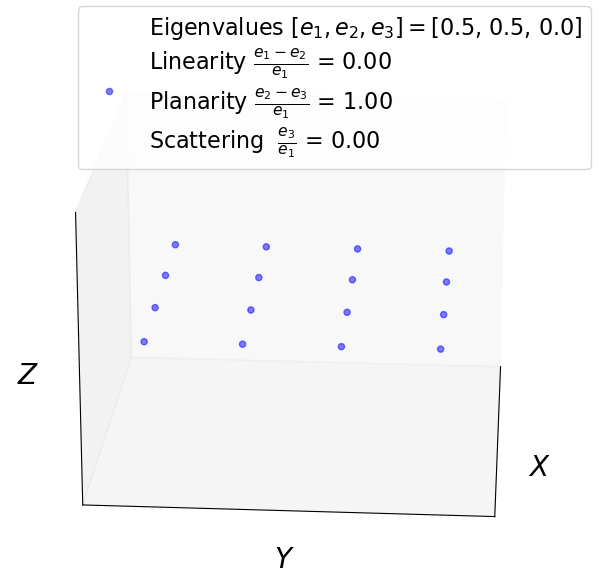
\includegraphics[width=0.48\textwidth]{fig/Planar System.png}
  \caption{Normalized Eigenvalues, Linearity, Planarity And Scattering Of A Linear And Planar Dataset.}
  \label{fig:Linear system}
\end{figure}

Furthermore for any combination where \(e_1 + e_2 \approx\) 100\% the points that make up the cluster must be confined to a 2D plane made up by the first and second eigenvector. This is true because \(e_3\) contributes approximately nothing towards explaining the variance and the cluster is almost fully explained by the two most important eigenvalues spanning a 2D plane. This feature of \textit{planar dimensionality} \(\lambda_{2D}\) can be expressed as low or close to zero \textit{scattering} \(S_\lambda\) in (\ref{eq:shannon 2D})
\begin{equation}
\label{eq:shannon 2D}
    \text{The dataset is }\lambda_{2D} \text{ if: } S_\lambda = \frac{e_3}{e_1} \approx \frac{e_3+ \epsilon}{e_1 + \epsilon} \approx 0
\end{equation}
if \(\epsilon\) is an infinitesimally small number to avoid any possible numerical division errors. These features can be taken advantage of by evaluating either the \(\lambda_{2D}\) directly for the cluster or by evaluating the specific Shannon Entropy given by (\ref{eq:shannon scattering})
\begin{equation}
\label{eq:shannon scattering}
    S_k = -L_\lambda\ln{(L_\lambda +\epsilon)} -P_\lambda\ln{(P_\lambda +\epsilon)} -S_\lambda\ln{(S_\lambda +\epsilon)}
\end{equation}
where \(S_k\) is the Shannon Entropy for a cluster given by the \(k\) number of nearest neighbours. \(S_k\) can in turn be optimized for the number \(k\) such that only points on the same surface is evaluated and thus removing the problems displayed in Figure \ref{fig:Sample Data-set with least squares}. Note that in theory the Shannon Entropy would optimize for a linear dimensional \(\lambda_{1D}\) system because the least uncertainty in any given 3D point cluster would be if \(e_1\) explained 100\% of the variance. In reality due to both measurement uncertainties and the nature of the objects that are scanned, such a scenario can't, or is extremely unlikely to occur when facing real datasets. There is still one scenario where this is true, and that is if only two points are evaluated, pairing only two points will always produce a \(\lambda_{1D}\) system simply from the fact that a straight line can be drawn through any two points provided they are not the same point. The optimization of \(S_k\) should then have a lower cutoff range at least above 2 in order to avoid this scenario, otherwise the ideal k would always be equal to 2. When this scenario is taken care of the least uncertainty in a cluster is then defined by one dimension higher where both \(e_1 \text{ and } e_2 > 0\). Meaning that for real datasets the Shannon Entropy optimizes for \(\lambda_{2D}\) systems.

Having optimized \(k\) from a range of e.g. [\(5 \to 40\)] the resulting \(S_k\) is a cluster of the initial selected point \(p_0\) and it's \(k\) nearest neighbours which in real practical scenarios should be the best \(\lambda_{2D}\) representation of the surface in which \(p_0\) lies. From this cluster a best-fit SVD plane can be constructed such that the material thickness can be determined.

From the \textit{Total Least Squares} page \cite{Total-Least-Squares} the SVD best-fit can be implemented as a plane constructed from the least significant, right singular  vector \(v_3\) and the initial selected point \(p_0\) by using equation (\ref{eq:Point Vector Plane}). From the SVD deconstruction of the 3D point cluster the resulting \(v\) vector in \(u\sum v\) contain much alike the eigenvectors the direction of the highest order explainable variance. This means that \(v_3\) is the best-fit vector orthogonal to the plane described by \(v_1 \text{ and } v_2\).\footnote{The best-fit SVD method is not expressed in it's entirety as this falls outside the scope of the thesis. The interested reader is referred to \cite{Total-Least-Squares} and \cite{3d-svd}.}
\clearpage

Combining the two presented methods and applying them to the simple dataset from (subsection \ref{sub:Euclidean Distance}) makes the \textit{Neighbourhood Optimized Planes} method capable of structuring local regions around a given point \(p_0\) where the surface can be expressed best as a \(\lambda_{2D}\) plane. The sensitivity towards changes in point density and point localisation is highly decreased as seen when comparing the results with the identical dataset in Figure \ref{fig:Sample Data-set with least squares} to Figure \ref{fig:Sample Dataset with Optimal Neighberhood Selection}. Furthermore the bias towards a certain orientation has been removed by introducing the SDV best-fit plane. 

\begin{figure}[H]
  \centering
  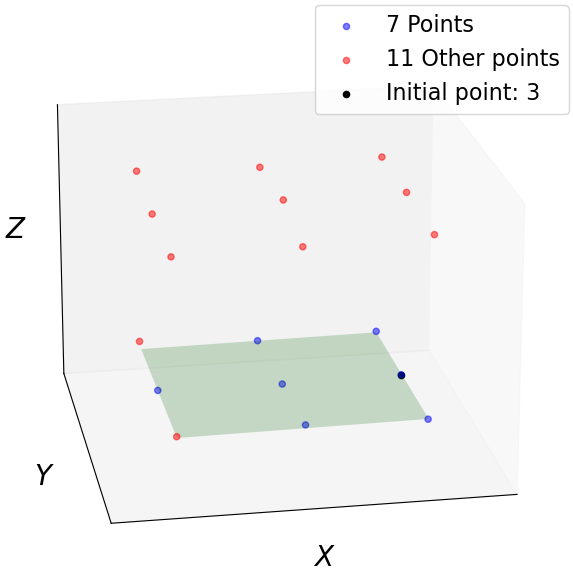
\includegraphics[width=0.40\textwidth]{fig/6 nearest points optimal.png}
  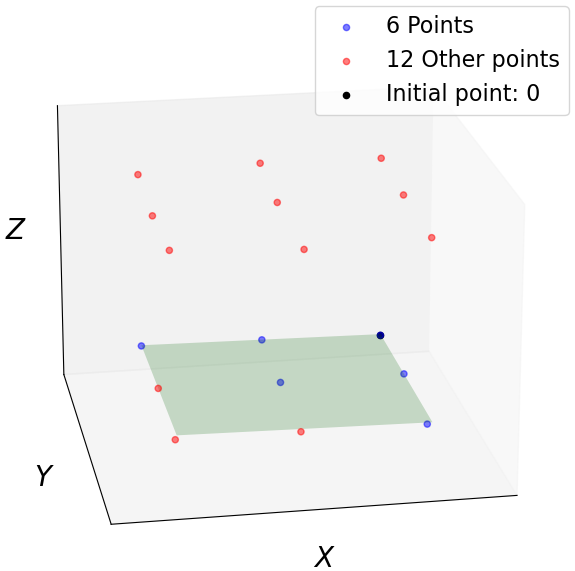
\includegraphics[width=0.40\textwidth]{fig/6 nearest points edge optimal.png}
  \caption{SVD Plane Fitting On 3D Sample Dataset With Varying \(p0\) And \(k\) Neighbouring Points.}
  \label{fig:Sample Dataset with Optimal Neighberhood Selection}
\end{figure}

The method satisfies the initial requirement from (subsection \ref{sub:General Point Cloud Methods}) such that it is invariable towards changes in \textit{point density} and \textit{orientations}. However the final step in the algorithm presented in (subsection \ref{sub:Parellel 2D Planes}) still has a reliance upon finding parallel planes, thus relying on a \textit{known} object \textit{shape}. 

\subsection{Material Thickness Optimized Plane Search}
\label{subsec:Material Thickness Search and Evaluation}
It is fairly simple to demonstrate why more complex systems can't be solved in this manner. Evaluating the material thickness across the 2D example in Figure \ref{fig:2D Material Thickness} the thickness varies along the X-axis as a result of the bottom surface not being flat. Picking the initial point \(B\), a plane can be constructed such that the local feature for the surface surrounding \(B\) is represented as a \(\lambda_{2D}\) plane. Investigating where the normal \(\vec{b}\) to the plane intersects with the other surface, a plane can be constructed in the same manner to fit the nearby local region. This plane will however not be parallel to the one in \(B\), nor will the length of the normal \(\vec{b}\) between them be the material thickness.

\begin{figure}[H]
  \centering
  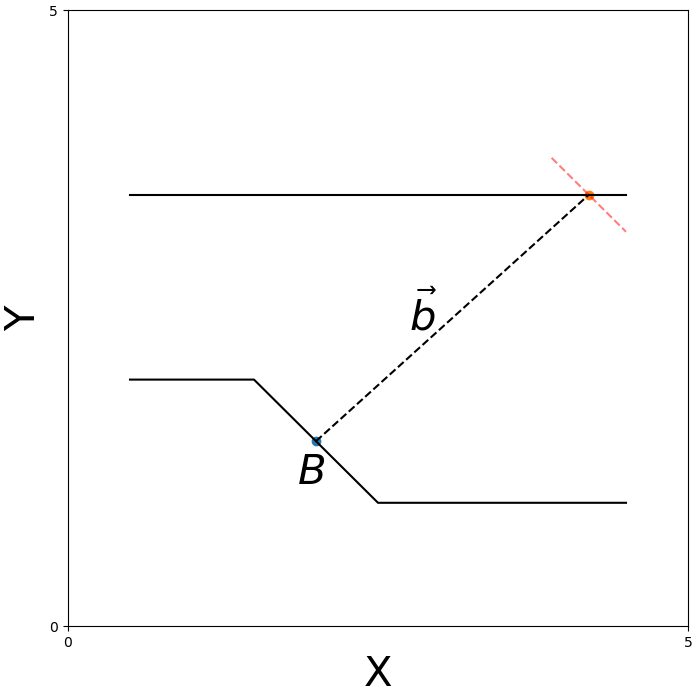
\includegraphics[width=0.40\textwidth]{fig/2D not parallel 1.png}
  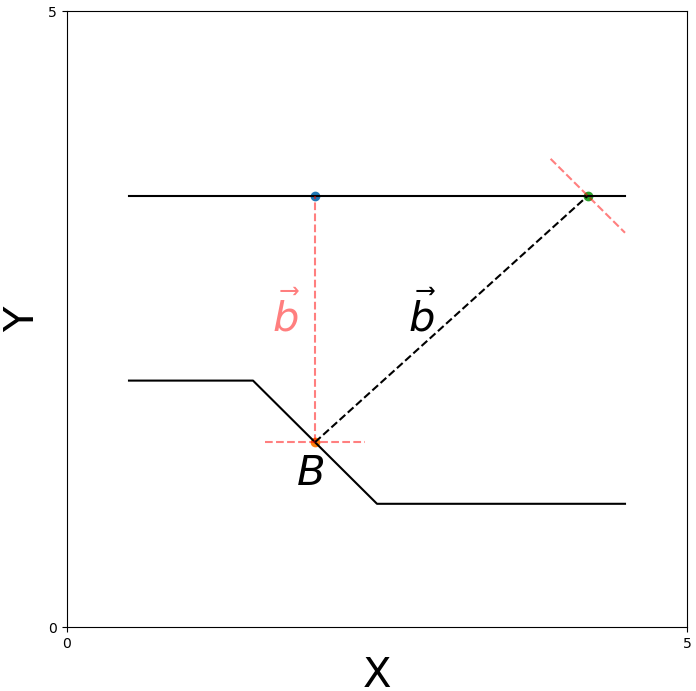
\includegraphics[width=0.40\textwidth]{fig/2D not parallel 2.png}
  \caption{2D Material Thickness From Point \(B\) By The Shortest Distance Plane Normal \(\vec{b}\) Search.}
  \label{fig:2D Material Thickness}
\end{figure}

In Figure \ref{fig:2D Material Thickness} the correct material thickness is the vector \textcolor{red}{\(\vec{b}\)}, notably this is a normal vector constructed from the intersection plane found in the initial search from point \(B\). This means that the following two part search algorithm (Listing \ref{lst:Material Thickness Search Algorithm}) can be carried out in order to ensure that the shortest distance is found. 

\begin{lstlisting}[mathescape, escapeinside={(*}{*)}, caption=Material Thickness Two Way Search Algorithm. , label={lst:Material Thickness Search Algorithm}]
Select an initial point $p_0$.
Determine the best $k$ nearest neighbours through $S_k$ (*(\ref{eq:shannon scattering}) *).
Construct a SVD best-fit plane for the cluster of $k$ points.
Use the plane normal $\vec{v}$ to determine the intersecting opposing surface.
From the intersected point, determine the best $k$ nearest neighbours by $S_k$.
Construct a SVD best-fit plane plane for the cluster of $k$ points.
Let the plane normal $\textcolor{red}{\vec{v}}$ intersect the first point $p_0$.
Calculate the euclidean distances of the two normal vectors.
Select the shortest distance as the material thickness.
\end{lstlisting}

The last hurdle to overcome is the fact that in a point cloud the plane normal is not guaranteed to intersect a point on the opposing surface. Here two methods can be implemented to determine the point closest to the theoretical intersected point.

The distance from any point \(p_n\) to the normal vector \(\vec{v}\) can be found through (\ref{eq:dist from point to line})
\begin{align}
    \label{eq:dist from point to line}
    dist & = \frac{\sqrt{((p_n - p_0)\times \vec{v})\cdot ((p_n - p_0)\times \vec{v})}}{\sqrt{\vec{v}\cdot \vec{v}}}
\end{align}
where \(p_0\) is the initial point, "\(\times\)" is the cross product and "\(\cdot\)" is the dot product. 
\clearpage

Similarly the angle between the normal vector \(\vec{v}\) and a vector formed by the initial point \(p_0\) and any point \(p_n\) is given by (\ref{eq:angle between vectors})

\begin{align}
\label{eq:angle between vectors}
    angle &= \frac{\arccos{(\vec{u_n}\cdot \vec{u})}*180}{\pi} \text{ , where} \\
    \vec{u} = \frac{\vec{v}}{\sqrt{\vec{v} \cdot \vec{v}}} &\text{ and }
    \vec{u_n} = \frac{\vec{(p_n - p_0)}}{\sqrt{\vec{(p_n - p_0)} \cdot \vec{(p_n - p_0)}}} \text{ .}
\end{align}

Both methods for finding the closest point \(p_n\) to the theoretical intersecting point have their advantages and disadvantages. Evaluating the distance to the normal means that points on either two planes can be selected as the closest point. Using this method thus means having to exclude at the very least the points \(k\) that made the original plane in order to find the correct intersection point. Depending on the point distribution this may be more or less than the \(k\) points, e.g. simple to calculate but hard to generalize. On the other hand the angle is periodical and dependant on the direction of the normal vector \(\vec{v}\). Meaning that the minimum value of \(abs(\arccos{(\vec{u_n}\cdot \vec{u})})\) and \(abs(\arccos{(\vec{u_n}\cdot \vec{u})} - \pi)\) has to be selected in (\ref{eq:angle between vectors}) in order to get the correct intersection point.

Implementing the material thickness algorithm from (Listing \ref{lst:Material Thickness Search Algorithm}) combined with the approximation for the closest intersection point through the minimum angle search the method is finally decoupled from all the dependencies presented in (subsection \ref{sub:General Point Cloud Methods}).

In order to demonstrate the method, two new datasets \(A\) and \(B\) are introduced, both \(A\) and \(B\) are comprised of 3D points structured randomly across two opposing disks. Unique for \(B\) is that the bottom disk has a step function along the distribution of the disk. \(A\) and \(B\) are demonstrated in Figure \ref{fig:3D dataset a and b}

\begin{figure}[H]
    \centering
    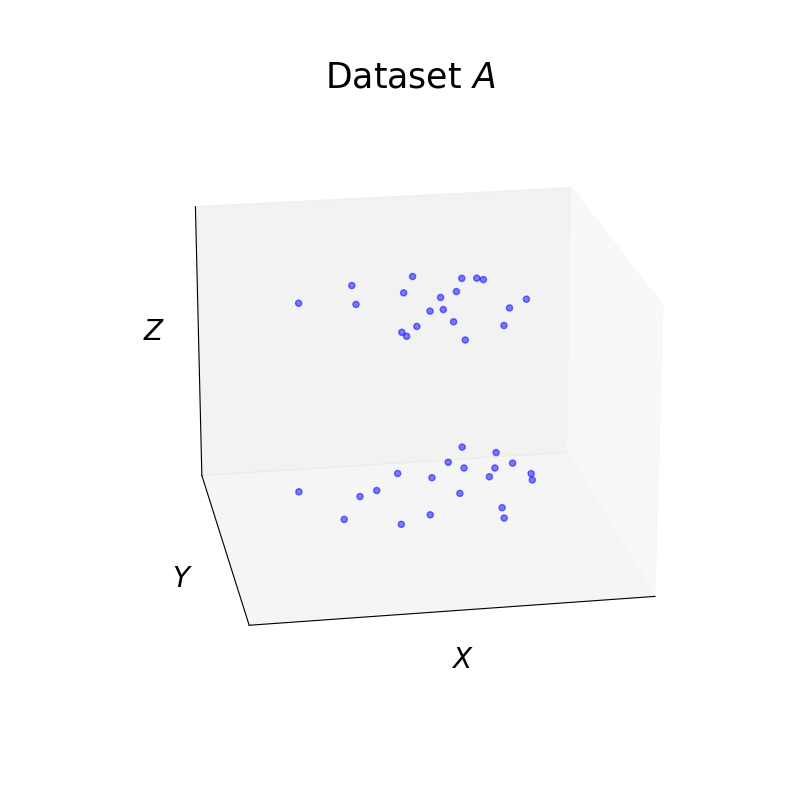
\includegraphics[width=0.40\textwidth]{fig/3D dataset A.png}
    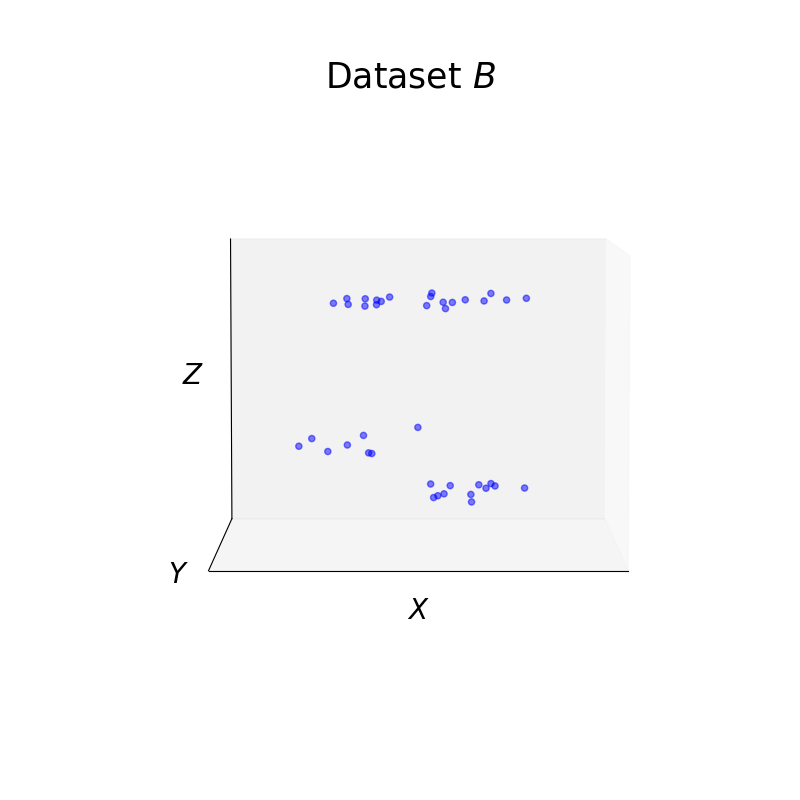
\includegraphics[width=0.40\textwidth]{fig/3D dataset B.png}
    \caption{Dataset \(A\) and \(B\) Comprised of Randomly Distributed 3D Points Along Two Opposing Disks.}
    \label{fig:3D dataset a and b}
\end{figure}


Applying the two way material thickness search algorithm from (Listing \ref{lst:Material Thickness Search Algorithm}) on dataset \(A\) using a randomly selected point as the starting point \(p_0\). The material thickness is initially evaluated to be 1.9922, whereas the second search reveals that there exist a better pairing which returns a material thickness of 1.9789 as demonstrated in Figure \ref{fig:Material Thickness Two Way Search Demonstrated on Dataset A}.

\begin{figure}[H]
  \centering
  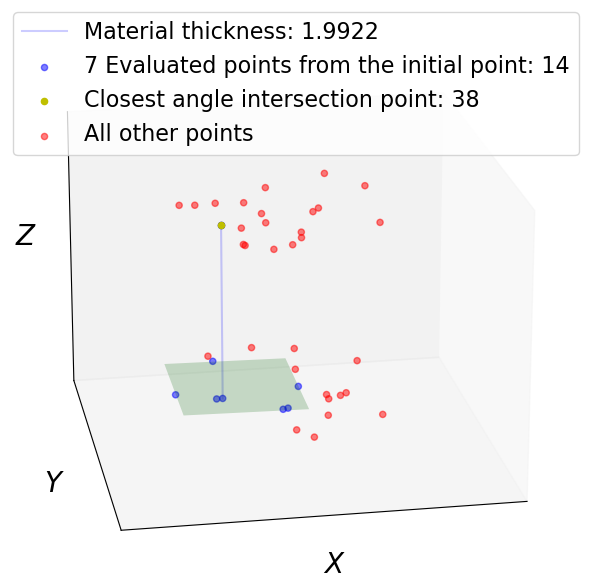
\includegraphics[width=0.35\textwidth]{fig/SVD Material Thickness Search 1.png}
  \hspace{0.5cm}
  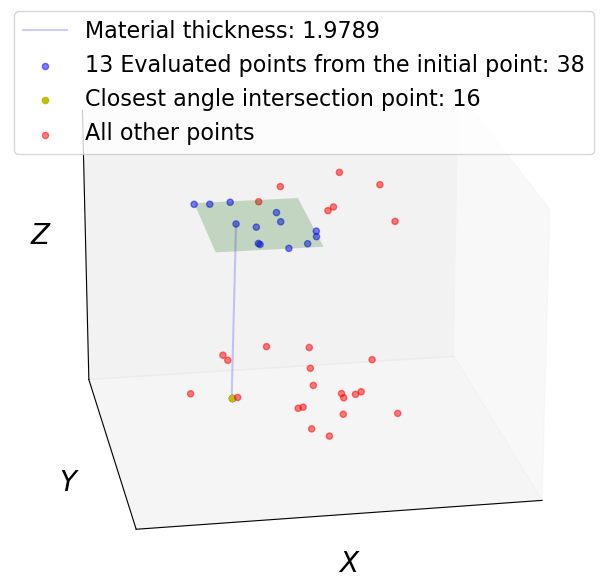
\includegraphics[width=0.35\textwidth]{fig/SVD Material Thickness Search 2.png}
  \caption{Material Thickness Two Way Search Demonstrated On Dataset \(A\).}
  \label{fig:Material Thickness Two Way Search Demonstrated on Dataset A}
\end{figure}

Likewise for dataset \(B\) a better approximation is found on the second search as shown in Figure \ref{fig:Material Thickness Two Way Search Demonstrated on Dataset B}.

\begin{figure}[H]
  \centering
  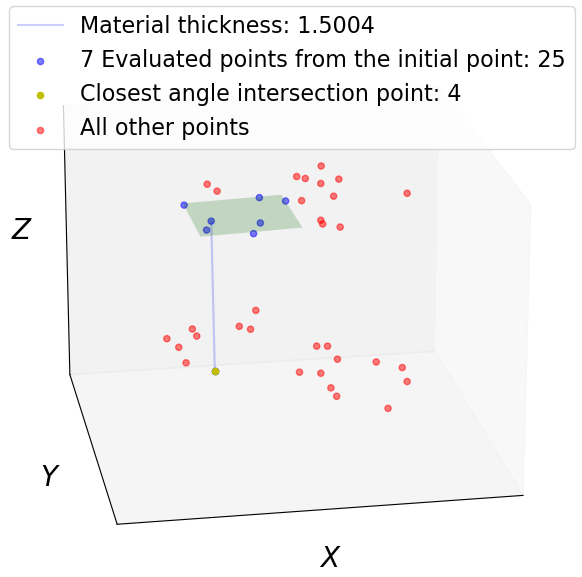
\includegraphics[width=0.35\textwidth]{fig/Material Thickness Optimal Neighbourhood Step Border Top.png}
  \hspace{0.5cm}
  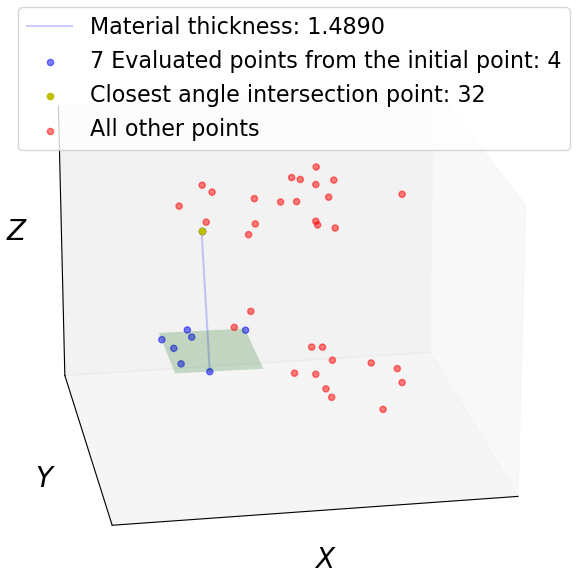
\includegraphics[width=0.35\textwidth]{fig/Material Thickness Optimal Neighbourhood Step Border Bottom.png}
  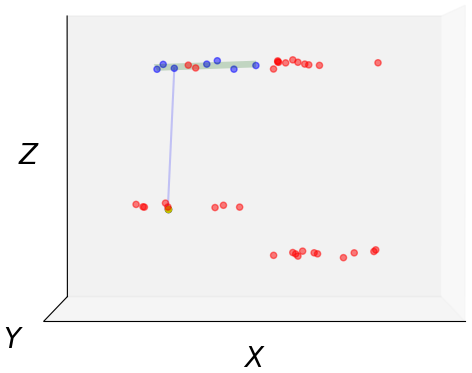
\includegraphics[width=0.30\textwidth]{fig/Material Thickness Optimal Neighbourhood Step Border Top 2.png}
  \hspace{1.15cm}
  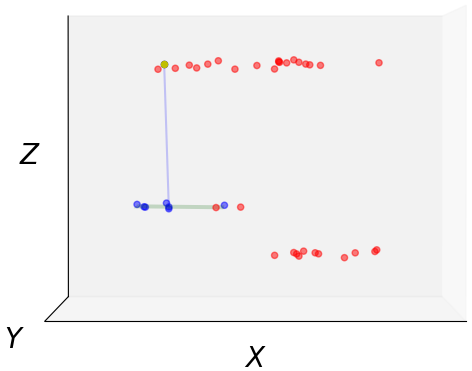
\includegraphics[width=0.30\textwidth]{fig/Material Thickness Optimal Neighbourhood Step Border Bottom 2.png}
  
  \caption{Material Thickness Two Way Search Demonstrated On Dataset \(B\).}
  \label{fig:Material Thickness Two Way Search Demonstrated on Dataset B}
\end{figure}


\section{ATOS Professional}
\label{sc:ATOS Professional}
The software solution for the GOM measurement cell is ATOS Professional, a 3D inspection and metrology system designed for use in ATOS 3D scanning systems. The most notable functionality of the software in respect to this thesis is it's capability of being scripted through the programs own script functions. This allows for inspections and operations of the scanned component data to be carried out autonomously in accordance with the script. The scripts are written in the programming language Python and are capable of doing any and/or all operations the software normally is capable of.\footnote{Notable functions are described in the project work AWA by Austefjord, R. 2020  \cite{Adaptive-Welding-Automation}.} While also having the possibility to introduce new functionality through programming.

\subsection{ATOS Professional Scripts}

To resolve the open point regarding autonomous digitization of components from AWA by Austefjord, R. 2020 \cite{Adaptive-Welding-Automation}, a script has to be developed in order to select the welding junctions of the components and calculate their material thickness.

\begin{wrapfigure}{r}{0.4\textwidth}
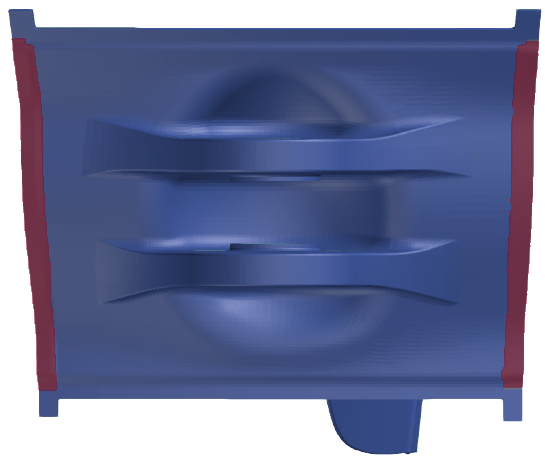
\includegraphics[width=0.9\linewidth]{fig/CAD Welding Junctions.png}
\caption{CAD Model Of A Mount-Strut With Welding Junctions Indicated In Red, Model In Courtesy Of GKN Trollhättan \cite{GKN_assets}.}
\label{fig:CAD model of a Mount-Strut}
\end{wrapfigure}

To achieve a suitable selection of the welding junctions some prior setup is required, notably custom Computer Aided Design (CAD) models can be made for each unique component type. Within these CAD models the welding junctions can be classified as predefined areas that the software easily can recognize once the CAD model is imported. An example of this is shown in Figure \ref{fig:CAD model of a Mount-Strut} where the red areas are the welding junctions for that component type. These areas can then easily be evaluated by the programs built in material thickness function and exported for use and storage. The python code to achieve the automated material thickness evaluation is described in Appendix (\ref{app:Software Source Code}).






\chapter{Results}
\label{ch:results}

As this thesis investigates the realm of 3D scanning as measurement system, 3D data structures, 3D data classification and evaluation as well as developing general frameworks and methods based upon known studies and methods. The results are divided into two sections in order to provide a clear overview of the work that has been done in the thesis, contrasted to how existing methods have been utilized. The division is structured by what is \textit{known} and what \textit{has been done}.

\section{Investigational Results}
In order to present general methods and frameworks for 3D scan data, four known data structures have been discussed on the terms of usability and functionality. Out of the four representations (\textit{Image}, \textit{Volumetric}, \textit{Meshes} and \textit{Point Clouds}) it has been determined through this thesis that for the goal of analyzing the datasets, the point cloud representation provide the best analytical base.

The 3D point cloud information has been investigated in order to determine the dependencies both with respects to the measurement systems as well as the originating object. The problems surrounding 3D scanning as a measurement system have been presented where a claim has been stated that in order for any particular applicable method to be truly general, it has to be capable of invariance towards \textit{point density}, \textit{orientation} and prior \textit{empirical} or \textit{heuristic knowledge}.

From the presented invariance claim, methods to remove the dependencies has been investigated in order to infer useful knowledge from the information within the datasets. Firstly a method for providing general data frameworks was considered in order to structure the otherwise unstructured and reference system dependant collection of 3D points. It has been shown through the thesis that any point cloud can be structured as a \textit{graph} framework, making it simple to classify and structure each point by their nearest neighbouring points as \textit{adjacency lists} through the known method of \textit{KD-Tree} structuring.

From the graph structure further knowledge can be inferred such as classifying local point clusters by their dimensionalities through known methods for eigenvalue analysis. These clusters can be found invariant to point densities, orientation or location through a minimization of the "uncertainty" entropy through the known \textit{Shannon Entropy} method.

\section{Development Results}
Utilizing the methods discussed in \textit{Investigational Results}, a general method for determining material thickness in unstructured 3D measurement data has been presented. Drawing inspiration from the human intuition and knowledge of what and how material thickness is determined, the method was developed from a point to point measurement of \textit{Euclidean Distance} to a complex \textit{Material Thickness Optimized Plane Search} algorithm. Importantly the final algorithm operates invariant towards \textit{point density}, \textit{orientation} and prior \textit{empirical} or \textit{heuristic knowledge}. However it is not infallible and have only been tested on simple fabricated 3D datasets which is discussed further in \textit{Discussion}.

A method for autonomously determining the material thickness through the ATOS Professional software has been presented where the scanned 3D data is compared to CAD models with predefined segments of interest. 

The methods have been implemented through code available in Appendix \ref{app:Software Source Code}.



% kan trekke frem 

% Establish method(s) for unstructured 3D measurement data evaluation and classification for TRF and general components.
\chapter{Conclusion}
\label{ch:conclusion}
For methods applied to 3D scan measurement data represented as \textit{point clouds} to truly be general, they have to be invariant to variations in \textit{point density}, \textit{orientation} and prior \textit{empirical} or \textit{heuristic knowledge}.

A general \textit{graph} framework can be built using \textit{KD-tree} clustering. Local clusters can be classified by their surrounding nearest points to form different dimensionality features such as \textit{Linearity} \(L_\lambda\), \textit{Planarity} \(L_\lambda\) and \textit{Scattering} \(L_\lambda\). These clusters can be defined from varying point densities through the optimization of the \textit{Shannon Entropy} for the normalized dimensionality features expressed as "pseudo probabilities".

Material thickness for low curvature objects can be determined through evaluating the distance between two opposing planes formed by the local clusters discovered by the \textit{Shannon Entropy} evaluation of the individual points. See the implemented algorithm in Listing \ref{lst:viz}.

Material thickness can be autonomously determined through the ATOS Professional software by comparing 3D scan data with predefined CAD models. See the implemented script in Listing \ref{lst:Thickness Automation}.

Functions, methods and scripts have in general been implemented through Python code available in Appendix \ref{app:Software Source Code}.

\chapter{Discussion}
\label{ch:discussion}
Due to the extremely broad goal of making a general solution applicable to any 3D point cloud dataset, the development had to be segmented into solving a subset of simpler/smaller problems rather than tackling everything at once. This means that for testing purposes the methods have been tested on appropriately challenging fabricated data in stead of real measurement data. There is a couple reasons for this, firstly it ensures that the method can be tested under a controllable environment. Secondly the results are intuitive and understandable compared to results from highly complex datasets. Maybe more importantly for the sake of development progress, inconsistencies and errors are simpler to handle because of the controllable and easier to understand test environment. Likewise due to the sheer size of the real datasets, the results from the tests can be produced in milliseconds as opposed to minutes or hours.

There has been done an effort in collecting real measurement data for three commonly used reference objects used in the aerospace manufacturing industry, a \textit{sphere}, a \textit{cylinder} and a \textit{slab}. These reference objects have known measurable properties such as diameter, length, width, depth, angle and run-out. However it has been known for quite some time that highly curved objects would pose at least in my perceivable theory, unsolvable problems for a general method. The reason is paradoxical in nature, taking a sphere as an example, the material thickness of a sphere is it's diameter which is the longest distance between two points on the sphere. This breaks the previously assumed notion that the material thickness is the shortest distance between two opposing surfaces. For these reasons both the spherical and cylindrical dataset was deemed unfit to evaluate the current model. The "square-ish" slab could be a good candidate to test the current model, however it was never tested because it's too large (43M 3D points). Reducing the size almost exactly equates to the same problem of the fabricated simple 3D dataset otherwise used, so this would be a needlessly complex operation for little benefit. Regardless the presented method will most assuredly fail for spherical or highly curved objects.

The two way material thickness search algorithm is somewhat clumsy and not the best solution. A better method for determining the closest point would be to let a sphere expand from the initial point \(p_0\) until it hits another point \(p_n\). This would ensure that the most optimal point would be selected every time. However since the sphere expands in all directions, the first point encountered would very likely be the neighbouring point on the same surface. This means that the method would have to know how to differentiate between points along the same surface and "other points of interest". A solution to this problem should be possible and is noted in \textit{Further Work}.

In the presented general material thickness method, SVD is used to best-fit a plane to the point cluster. Notably this might be needlessly complex since the only value extracted from the SVD is the least significant right singular value. This could likewise be done by selecting the least significant eigenvector in e.g. a PCA decomposition.


\(\lambda_{2D}\) which is utilized in (subsection \ref{sub:Neighbourhood optimized SVD Best-Fit Planes}) could be expressed more accurately as (\ref{eq:lambda 2D})
\begin{equation}
\label{eq:lambda 2D}
    \lambda_{2D} = \frac{e_3}{e_1 + e_2} \approx \frac{e_3+ \epsilon}{e_1 +e_2 + \epsilon} \approx 0
\end{equation} though this formulation can't be used in the Shannon Entropy equation. This is because the evaluated probabilities has to sum up to 1, this is of course achievable by for example including the "\textit{not} \(\lambda_{2D}\)" such that (\ref{eq:lambda 2D 2}) 
\begin{equation}
\label{eq:lambda 2D 2}
    \frac{e_3}{e_1 + e_2} + \frac{e_1 + e_2 -e_3}{e_1 + e_2} = 1 \text{ .}
\end{equation}
However it is difficult to express what scenario "\textit{not} \(\lambda_{2D}\)" refers to or in other words it does a poor job of describing the dimensionality present if the data is not \textit{planar dimensional} \(\lambda_{2D}\). It is also unknown if the natural tendency within a dataset is to have a lower value for "\textit{not} \(\lambda_{2D}\)" than \(\lambda_{2D}\) or vice versa. Notably \(\frac{e_3}{e_1} \approx \frac{e_3}{e_1 + e_2}\) because \(e_1 \geq e_2\) and \(e_1 \gg e_3\) meaning this simplification introduces very little error.

\section{Further Work}
\label{sec:Further Work}
From the work done in the thesis many new questions have arisen which could prove insightful in order to improve upon the presented solutions.

The broad field of \textit{graph theory} contain many elegant and computational cost efficient algorithms. Many of the problems attempted solved in this thesis might be possible to rephrase into problems solvable by such algorithms. Thus a study into the capabilities of \textit{graph theory} may improve the methods substantially.

Due to a design choice in the implementation process of the material thickness algorithm, the \textit{Shannon} entropy is optimized using a brute force approach, ranging from \(5 \to 40\). This is done because other optimizers such as \textit{Newton-Cotes} or the \textit{Bernt's Algorithm} do not allow for integer solutions. Such algorithms would, and in fact does produce errors if they do not get to investigate the numerical realm between two whole numbers. However it makes no sense to look at 6 and a half nearby points, meaning the algorithm gets stuck at the first local minima it finds. The brute function works decently but is not truly invariant to point density changes since the roof of the search is capped. It is also slow since it has to evaluate 35 points every time the function is called. Here a better optimizer should be implemented.

Similarly when the material thickness algorithm searches for the smallest angle difference to the ideal "\(p_n\) intersection", brute force is applied as the optimizer. There seems to be no good way of improving such a search which means that currently the algorithm has to evaluate every point in the dataset, twice because the algorithm is repeated when finding the second material thickness back towards the initial point \(p_0\). Here there might be vastly better ways of doing such a search if the problem could be formulated as a graph problem.

SVD is in this thesis only used to find the least significant right singular value in the local cluster. It should be worth investigating whether more useful insight might be derived from other parts of the decomposition. SVD might also be useful for analysing the whole dataset or groups of clusters, reducing the structure or determining the most important features (highest rank sigmas), etc\dots

For highly curved objects it could be a posibility to best-fit a sphere and use the tangent plane intersecting the initial point \(p_0\) to determine the normal direction of the material thickness. For complete spheres datasets, best-fit spheres could also give the radius, e.g. material thickness directly from the formula.

It could be worth investigating methods to triangulate the dataset and subsequently evaluating the triangles. It was noted while reviewing mesh Grid structures in dialogue with Associate Proff. Håkon Viumdal and Proff. Ola Marius Lysaker that in planar areas, the triangles usually had similar angles between the edges. In areas with high curvature or close to edges there would be considerably more sharp angles, where one angle would be very small compared to the other two. There then might be an analytical benefit from investigating the triangles angles and their edge lengths in order to see if any useful information could be extrapolated.


% A dummy command that causes all bibliographyentries to be displayed
% even though there were not cited in the document. Used for demonstration
% purposes only in this template file.
~\nocite{*}


% The bibliography should be displayed here...
\printbibliography[heading=bibintoc]
% You rather like to call the bibliography "References"? Then use this instead:
%\printbibliography[heading=bibintoc, title={References}]

\appendix
%\renewcommand{\appendixname}{Paper} %% So we get 'Paper X' displayed instead

\chapter{Software Source Code}
\label{app:Software Source Code}
Below the software developed through the master thesis are presented. The code is documented inline and with a short description preceding the code listing.


\section{GOM Inspect Suite Script}
\label{app:GOM Inspect Suite Script}
The following script in (Listing \ref{lst:Point Collection}) may be used in the ATOS Professional GOM Inspect Suite in order to extract both the scanned point cloud and it's triangulated mesh grid from an element named "Name of Element" (exchangeable in the code).

\begin{lstlisting}[language=Python, caption=GOM Point Collection, label={lst:Point Collection}]
import numpy as np
import gom

points = np.array(gom.app.project.actual_elements[
                      'Name of Element'].data.coordinate)
tri = np.array(gom.app.project.actual_elements[
                        'Name of Element'].data.triangle)
print(points)
print("The shape of the points array: {}\nThe size of the "
      "points array: {}".format(np.shape(points), np.size(points)))

print(tri)
print("The shape of the triangle array: {}\nThe size of the "
      "triangle array: {}".format(np.shape(tri), np.size(tri)))
\end{lstlisting}

\clearpage
\section{GOM Inspect Suite Automation Script}
\label{app:GOM Inspect Suite Automation Script}

The following script may be used to open, establish and extract the material thickness across any predefined area by location or name through the "gom.script.selection3d.select\_patch" function.

\begin{lstlisting}[language=Python, caption=GOM Automation, label={lst:Thickness Automation}]
import gom
import numpy as np


"""Import cad model and rename"""
gom.script.sys.import_stl (
	bgr_coding=True, 
	body_split='no_color', 
	files=['C:/Users/Ruben/School/IIA Master/03_02 Master Thesis/ATOS Professional/Mounts/VAN_Y00001035_07.stl'], 
	geometry_based_refining=False, 
	import_mode='clipboard', 
	length_unit='mm', 
	stl_color_bit_set=False, 
	target_type='cad_body')

gom.script.part.create_new_part (name='Mount-Strut-CAD')

gom.script.part.add_elements_to_part (
	delete_invisible_elements=True, 
	elements=[gom.app.project.clipboard.nominal_elements['VAN_Y00001035_07']], 
	import_mode='new_elements', 
	part=gom.app.project.parts['Mount-Strut-CAD'])


"""Import Mesh and rename"""

gom.script.sys.import_stl (
	bgr_coding=True, 
	files=['C:/Users/Ruben/School/IIA Master/03_02 Master Thesis/ATOS Professional/Scans/31860513_GUK905HA.stl'], 
	geometry_based_refining=False, 
	import_mode='clipboard', 
	length_unit='mm', 
	stl_color_bit_set=False, 
	target_type='mesh')

gom.script.part.create_new_part (name='Mount-Strut-Mesh')

gom.script.part.add_elements_to_part (
	delete_invisible_elements=True, 
	elements=[gom.app.project.clipboard.actual_elements['31860513_GUK905HA']], 
	import_mode='new_elements', 
	part=gom.app.project.parts['Mount-Strut-Mesh'])
	


"""Prealign"""
CAD_ALIGNMENT=gom.script.alignment.create_prealignment (
	computation_mode='normal', 
	compute_additional_bestfit=True, 
	name_expression='Prealignment', 
	parent_alignment=gom.app.project.parts['Mount-Strut-Mesh'].original_alignment, 
	part=gom.app.project.parts['Mount-Strut-Mesh'], 
	target_element=gom.app.project.parts['Mount-Strut-CAD'].nominal)

"""Set visability of Mesh off"""
gom.script.cad.hide_element (elements=[gom.app.project.parts['Mount-Strut-CAD'].actual])

"""Select welding junction"""



"""Mimic select CAD feature
gom.script.selection3d.select_patch (
	coordinate=gom.Vec3d (7527.677051, 803.1583909, 178.786535), 
	target=gom.app.project.parts['Mount-Strut-CAD'].nominal)
"""


"""Create material thickness"""
MCAD_ELEMENT=gom.script.comparison.create_multiple_material_thickness (
	max_angle_between_normals=0.436332313, 
	max_opening_angle=1.047197551, 
	max_thickness=6.0, 
	min_thickness=1.0, 
	name='Material Thickness Welding Junction Right 1')
	
Material_thickness = np.array(gom.app.project.actual_elements['Material Thickness Welding Junction Right 1'].data.coordinate)

print(Material_thickness)
print(Material_thickness.shape)
print(Material_thickness.size)

\end{lstlisting}
\clearpage
\section{Methods}
\label{app:Methods}
From the theoretical methods used throughout the thesis the vast majority has been implemented through Python code in the following (Listing \ref{lst:Methods}). The code has been developed in Python with some added features for ease of visualization. The code is presented piece-wise as functions for solving the different problems faced in the methods. The functions have been commented with intended input and output such that they may be used separately from any one method. An example of use is given in (Listing \ref{lst:viz}).

\begin{lstlisting}[language=Python, caption=Methods implemented in code, label={lst:Methods}]
import numpy as np
from scipy.spatial import KDTree
from scipy.optimize import brute


def generate_points(xx, yy, zz):
    """
    Function for creating a 3D-box of evenly distributed points.
    :param xx: the desired z dimensionality.
    :param yy: the desired y dimensionality.
    :param zz: the desired x dimensionality.
    :return: coordinates: a numpy array containing the 3D coordinates
    for the points.
    """
    coordinates = []
    for z in range(zz):
        for y in range(yy):
            for x in range(xx):
                coordinates.append("{} {} {}".format(x, y, z))
    coordinates = [w.split(' ') for w in coordinates]
    coordinates = np.asarray(coordinates).astype(np.float)
    coordinates = coordinates + ((np.asarray(np.random.rand(18, 3)) - 
                                  0.5) * 0.05)
    coordinates = coordinates * [1, 1, 2]
    return coordinates


def generate_points_disk(number, radius, offset):
    """
    Function for generating randomly distributed 3D points along a disk.
    :param number: The desired number of points.
    :param radius: The radius of the disk.
    :param offset: The offset in the z direction.
    :return: A numpy array containing the 3D coordinates for the points.
    """
    r = np.random.uniform(low=0, high=radius, size=number)
    theta = np.random.uniform(low=0, high=2 * np.pi, size=number)
    noise = np.random.uniform(low=-0.05, high=0.05, size=number)

    x = np.sqrt(r) * np.cos(theta)
    y = np.sqrt(r) * np.sin(theta)
    z = ([offset] * number) + noise
    return np.asarray(list(zip(x, y, z)))


def generate_plane_svd(points):
    """
    Function for fitting a plane to a set of points by the Singular 
    Value Decomposition method.
    :param points: A collection of points (x,y,z) that should be
    considered to find the best-fit plane.
    :return: x, y, z and normal: Returns the plane function z bounded 
    by the max/min values of x and y structured in a meshgrid(xx, yy)
    for graphing. Returns the normal to the plane.
    """
    # defining the domain of the plane
    max_x = np.max(points[:, 0])
    max_y = np.max(points[:, 1])
    min_x = np.min(points[:, 0])
    min_y = np.min(points[:, 1])
    x, y = np.meshgrid([min_x, max_x], [min_y, max_y])  
    # Note that the meshgrid is bounded by the x and y values, 
    # meaning that for planes orthogonal to the xy-plane this will 
    # produce a very bad visualization.

    # centering the data.
    centroid = points.mean(axis=0)
    points = points - centroid
    u, sigma, v = np.linalg.svd(points)
    normal = v[2]
    d = normal[0] * centroid[0] + normal[1] * centroid[1] + normal[2] \
        * centroid[2]

    z = (-normal[0] * x - normal[1] * y + d) * 1. / normal[2]
    return x, y, z, normal
    # Reference:
    # https://stackoverflow.com/questions/53591350/plane-fit-of-3d-points-with-singular-value-decomposition
    # https://math.stackexchange.com/questions/2810048/plane-fitting-using-svd-normal-vector


def generate_plane_lstsq(points):
    """
    Function for fitting a plane to a set of points by the least  
    squares method.
    :param points: A collection of points (x,y,z) that should be
    considered to find the best-fit plane.
    :return: x, y, z and normal: Returns the plane function z 
    bounded  by the max/min values of x and y structured in a 
    meshgrid(xx, yy) for graphing. Returns the normal to the plane.
    """
    matrix = np.column_stack((points[:, 0], points[:, 1], 
                              np.ones(points[:, 0].size)))
    (a, b, c), residual, rank, s = \
        np.linalg.lstsq(matrix, points[:, 2], rcond=None)
    normal = unit_vector(np.asarray([a, b, -1]))
    # defining the domain of the plane
    max_x = np.max(points[:, 0])
    max_y = np.max(points[:, 1])
    min_x = np.min(points[:, 0])
    min_y = np.min(points[:, 1])
    # creating a point in the plane
    point = np.array([0.0, 0.0, c])
    d = -point.dot(normal)
    x, y = np.meshgrid([min_x, max_x], [min_y, max_y])
    z = (-normal[0] * x - normal[1] * y - d) * 1. / normal[2]
    # Comment regarding non-linear plane:
    # https://gist.github.com/amroamroamro/1db8d69b4b65e8bc66a6
    return x, y, z, normal


def unit_vector(vector):
    """
    Function for finding the unit vector of a vector.
    :param vector: The original vector.
    :return: The unit vector of the vector.
    """
    return vector / np.sqrt(vector.dot(vector))


def vector_3d(p1, p2):
    """
    Function for substracting one point/vector from another.
    :param p1: (x_a, y_a, z_a)
    :param p2: (x_b, y_b, z_b)
    :return: ((x_b - x_a), (y_b - y_a), (z_b - z_a))
    """
    return p2 - p1


def euclidean_distance(p1, p2):
    """
    Function for calculating the euclidean distance between two points.
    :param p1: Point A
    :param p2: Point B
    :return: The euclidean distance between point A and B.
    """
    vector = vector_3d(p1, p2)
    return np.sqrt(vector.dot(vector))


def angle_between_vectors(vector1, vector2):
    """
    Function for finding the angle between two vectors by applying
    the common formula : angle = arccos(vector1 dot vector2 /
    magnitude(vector1) * magnitude(vector2)).
    :param vector1: The first vector.
    :param vector2: The second vector.
    :return: The radian and angle between the two vectors.
    """
    v1 = unit_vector(vector1)
    v2 = unit_vector(vector2)

    radians = np.arccos(np.clip(np.dot(v1, v2), -1.0, 1.0))
    angle = radians * 180 / np.pi

    return radians, angle


def brute_optimal_angle(data_set, point, normal):
    """
    Function for determining the optimal angle based on brute force 
    optimization.
    :param data_set: Data of (x,y,z) values / points to be evaluated.
    :param point: Point of origin.
    :param normal: The normal direction the points should be 
    evaluated  against.
    :return: The point in data_set that lie closest in terms of 
    angle  to the origin point.
    """
    def radians(n):
        v1 = unit_vector(vector_3d(point, data_set[int(n)]))
        v2 = unit_vector(normal)
        radian = min(np.arccos(np.clip(np.dot(v1, v2), -1.0, 1.0)), 
        abs(abs(np.arccos(np.clip(np.dot(v1, v2), -1.0, 1.0))) - np.pi))
        return radian

    result = brute(radians, (slice(1, data_set.shape[0], 1),))
    return data_set[int(result[0])]


def brute_optimal_distance(data_set, point, normal):
    """
        Function for determining the optimal distance based on brute
        force optimization.
        :param data_set: Data of (x,y,z) values / points to be evaluated.
        :param point: Point of origin.
        :param normal: The normal direction the points should be  
        evaluated against.
        :return: The point in data_set that lie closest in terms of 
        distance to the normal vector.
        """
    def dist(n):
        cross_product = np.cross((data_set[int(n)] - point), normal)
        distance = np.sqrt(cross_product.dot(cross_product)) /  \
                   np.sqrt(normal.dot(normal))
        return distance

    result = brute(dist, (slice(1, data_set.shape[0], 1),))
    return data_set[int(result[0])]


def flatten_2d(data):
    """
    Function for reducing a numpy array down to two dimensions.
    :param data: A numpy array of n>2 dimensions.
    :return: A numpy array of n <= 2 dimensions.
    """
    return data.reshape(-1, data.shape[-1])


def pca(points):
    """
    Function for Principle Component construction for further analysis.
    :param points: An array of points to be evaluated.
    :return: The Eigenvalues and Eigenvectors of the data. The
    centered data, the mean and the covariance matrix.
    """
    mean = np.mean(points, axis=0)
    data = (points - mean)
    matrix = np.cov(data.T)
    eigenvalues, eigenvectors = np.linalg.eig(matrix)
    return eigenvalues, eigenvectors, data, mean, matrix


def kd_tree(data):
    """
    Function for creating a KD-tree for the given data.
    :param data: The data to be structured in a KD-tree structure.
    :return: The data structured in a KD-tree.
    """
    return KDTree(data)


def neighborhood_selection(tree, data_set, initial_point):
    """
    Function for finding the best neighbourhood point cluster selection.
    :param tree: KD-tree of the data
    :param data_set: The dataset to be evaluated, this is the same  
    dataset as the KD-tree is structured by.
    :param initial_point: The initial point where the neighbourhood 
    should be optimized around.
    :return: S_k, the optimal number of k nearest neighbours.
    """
    def shannon_entropy(points):
        epsilon = np.finfo(float).eps
        cov_matrix = np.cov(points.T)
        eigen_value, eigen_vector = np.linalg.eig(cov_matrix)
        idx = eigen_value.argsort()[::-1]
        eigen_value = eigen_value[idx]
        sum = eigen_value[0] + eigen_value[1] + eigen_value[2]
        eigen_value = eigen_value / sum
        linearity = (eigen_value[0] - eigen_value[1]) / (
                eigen_value[0]  + epsilon)
        planarity = (eigen_value[1] - eigen_value[2]) / (
                eigen_value[0]  + epsilon)
        scattering = eigen_value[2] / (eigen_value[0] + epsilon)
        shannonentropy = (- linearity * np.log(linearity + epsilon)
                          - planarity * np.log(planarity + epsilon)
                          - scattering * np.log(scattering + epsilon))
        return shannonentropy

    def query(n):
        distances, nearest_neighbours = \
            tree.query([data_set[initial_point]], k=int(n))
        return shannon_entropy(flatten_2d(data_set[nearest_neighbours]))

    result = brute(query, (slice(5+1, 18+1, 1),))  
    # optimizes the minimum local solution within the given bounds  
    # using brute force.
    # result = minimize_scalar(query, bounds=(5, 10), method='bounded')  
    # optimizes the minimum local solution within the given bounds  
    # using Bernt's Algorithm.
    return result[0]


def general_shannon_entropy(points):
    """
    Function for evaluating a collection of points (x,y,z) in terms
    of local features and entropy.
    :param points: A cluster of 3D coordinates (x,y,z)
    :return: The Covariance Matrix, Eigenvalues, Eigenvectors,
    Linearity, Planarity, Scattering, Omnivariance, Anisotropy,
    Curvature, Sum Eigenvalues and the Eigenentropy.
    """
    epsilon = np.finfo(float).eps
    cov_matrix = np.cov(points.T)
    eigen_value, eigen_vector = np.linalg.eig(cov_matrix)
    idx = eigen_value.argsort()[::-1]
    eigen_value = eigen_value[idx]
    eigen_vector = eigen_vector[:, idx]
    sum = eigen_value[0] + eigen_value[1] + eigen_value[2]
    eigen_value = eigen_value/sum
    linearity = (eigen_value[0] - eigen_value[1]) / (eigen_value[0] 
                                                     + epsilon)
    planarity = (eigen_value[1] - eigen_value[2]) / (eigen_value[0] 
                                                     + epsilon)
    scattering = eigen_value[2] / (eigen_value[0] + epsilon)
    omnivariance = abs(eigen_value[0] * eigen_value[1] * 
                       eigen_value[2])**(1./3.)
    anisotropy = (eigen_value[0] - eigen_value[2]) / (eigen_value[0] 
                                                      + epsilon)
    curvature = eigen_value[2]/(eigen_value[0] + eigen_value[1] 
                                + eigen_value[2] + epsilon)
    sum_eigenvalues = eigen_value[0] + eigen_value[1] + eigen_value[2]
    eigenentropy = (- eigen_value[0] * np.log(eigen_value[0] + epsilon)
                    - eigen_value[1] * np.log(eigen_value[1] + epsilon)
                    - eigen_value[2] * np.log(eigen_value[2] + epsilon))
    shannonentropy = (  - linearity * np.log(linearity + epsilon)
                        - planarity * np.log(planarity + epsilon)
                        - scattering * np.log(scattering + epsilon))

    return cov_matrix, eigen_value, eigen_vector, linearity, \
           planarity, scattering, omnivariance, anisotropy,  \
           curvature, sum_eigenvalues, eigenentropy, shannonentropy
\end{lstlisting}

\begin{lstlisting}[language=Python, caption=Material thickness example use of Methods, label={lst:viz}]
import Methods
import matplotlib.pyplot as plt
import numpy as np
from mpl_toolkits.mplot3d import Axes3D


def material_thickness_example(initial_point=10):
    """
    Function for demonstrating the use of different functions in
    Methods.
    :param initial_point: The initial point, default is 10.
    """
    lower_bound = Methods.generate_points_disk(20, 1, 0)
    upper_bound = Methods.generate_points_disk(20, 1, 2)
    all_points = np.concatenate((lower_bound, upper_bound), axis=0)
    general_kd_tree = Methods.kd_tree(all_points)

    number_of_nearest_neighbours = int(Methods.neighborhood_selection(
        general_kd_tree, all_points, initial_point))
    distances, nearest_neighbours_index = general_kd_tree.query(
        [all_points[initial_point]], k=number_of_nearest_neighbours)
    nearest_neighbours_points = Methods.flatten_2d(
        all_points[nearest_neighbours_index])
    # *least_squares_plane, least_squares_normal =
    # Methods.generate_plane_lstsq(nearest_neighbours_points)
    # *least_squares_plane, least_squares_normal =
    # Methods.generate_plane_pca(nearest_neighbours_points)
    *least_squares_plane, least_squares_normal = \
        Methods.generate_plane_svd(nearest_neighbours_points)
    reduced_points = np.delete(all_points, [nearest_neighbours_index], 0)
    smallest_angle_point = Methods.brute_optimal_angle(
        reduced_points, all_points[initial_point], least_squares_normal)
    euclidean_distance = Methods.euclidean_distance(
        all_points[initial_point], smallest_angle_point)

    plt3d = plt.figure(figsize=(8, 8)).gca(projection='3d')
    plt3d.set_xlim3d(-1.5, 1.5)
    plt3d.set_ylim3d(-1.5, 1.5)
    plt3d.set_zlim3d(-0.5, 2.5)
    plt3d.set_xlabel('$X$', fontsize=20)
    plt3d.set_ylabel('$Y$', fontsize=20)
    plt3d.set_zlabel('$Z$', fontsize=20)
    plt3d.set_xticks([])
    plt3d.set_yticks([])
    plt3d.set_zticks([])
    plt3d.view_init(elev=20, azim=80)
    plt3d.scatter(*nearest_neighbours_points.T, c='b', marker='o',
    alpha=.5, label='{} Evaluated points from the initial point: '
                    '{}'.format(number_of_nearest_neighbours,
                                    initial_point))
    plt3d.plot_surface(*least_squares_plane, color='g', alpha=.2,
                       linewidth=0, zorder=1)
    plt3d.scatter(*smallest_angle_point.T, color='b')
    plt3d.scatter(*smallest_angle_point.T, color='y', label=
    'Closest angle intersection point: {}'.format(
        np.where(all_points == smallest_angle_point)[0][0]))
    matrix = np.asarray(list(zip(
        all_points[initial_point],  smallest_angle_point)))
    plt3d.plot3D(*matrix, color='b', alpha=.2, label=
    'Material thickness: {0:.4f}'.format(euclidean_distance))
    dataset_removed = np.delete(reduced_points,
    [np.where(reduced_points == smallest_angle_point)[0][0],
     np.where(reduced_points == smallest_angle_point)[0][0]], 0)
    plt3d.scatter(*dataset_removed.T, color='r', alpha=.5, label=
    'All other points')
    plt.legend(prop={"size": 16})
    plt.show()


if __name__ == '__main__':
    material_thickness_example()

\end{lstlisting}

\clearpage

\section{Cover Image}
\label{sc:Cover Image}
For the cover image I wanted to create a visible connection between my previous work related to the manufacturing of TRF's to the more general research on point clouds. To achieve this I wanted to repurpose the original grid-line TRF view as a reminder of where the work originated and gradually morph the image into a collection of points to indicate and introduce the current work. The shift goes from right to left in adherence to natural reading patterns generally used in "western civilisations" since this has given us a basic understanding/interpretation of progress forward in time going from right to left. As opposed to some "eastern civilisations" where the reading pattern is left to right and the opposite assumption holds.

\begin{figure}[H]
  \centering
  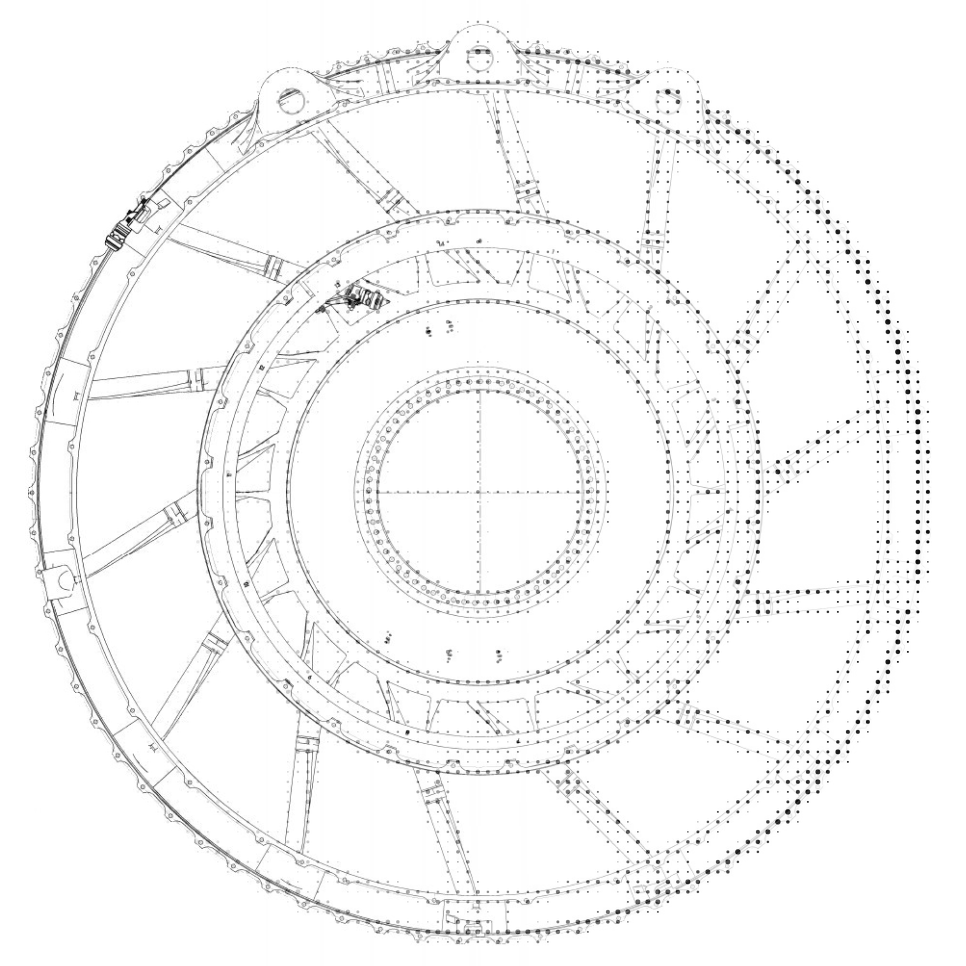
\includegraphics[width=0.45\textwidth]{fig/TRF Points 2.png}
  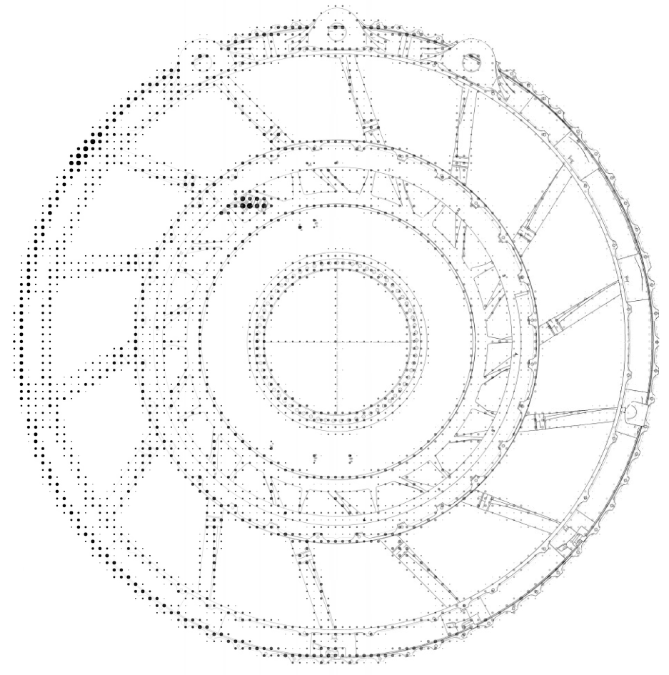
\includegraphics[width=0.44\textwidth]{fig/Points Inverted.png}
  \caption{Comparison Of Gradients From Left To Right / Right To Left.}
  \label{fig:Comparison of Gradients}
\end{figure}

There was two steps in creating this image, firstly the base image had to be represented as a collection of points. This was achieved through image processing in Python, mainly based upon the library composed by Phil Gyford \cite{Halftones}. 

A very quick and dirty introduction of how the code works is that you section the image into a fixed size grid of \(n \text{by} m\) size. Then you evaluate the content of each "box" within the grid and from that determine an appropriate size and colour of a circle that you will fill within that box. Generally speaking, if the original box was entirely yellow, it would result in a large yellow circle, if it was half yellow and half blue the circle would be green and if it was half yellow and half white, the circle would be yellow with a smaller radius.

The result is then an increase in contrast and reduction in resolution since darker colors are exaggerated and more empty space is introduced.

To achieve the result I had in mind I had to make some improvements mainly on how the content of the boxes was evaluated, how the circle color and radius was calculated and whether the background should be black filled with white circles or the background should be white filled with black circles.

The Python code for the halftone is listed in Listing \ref{lst:Gray-scale Halftone}.

\begin{lstlisting}[language=Python, caption=Gray-scale Halftone., label={lst:Gray-scale Halftone}]
import os
import sys
import numpy as np
from PIL import Image, ImageDraw, ImageStat


class Halftone(object):
    def __init__(self, path):
        """
        path is the path to the image we want to halftone.
        """
        self.path = path

    def make(self, sample=10, scale=1, filename_addition="_halftoned",
             angles=[0, 15, 30, 45]):
        """
        Leave filename_addition empty to save the image in place.
        Arguments:
            sample: Sample box size from original image, in pixels.
            scale: Max output dot diameter is sample * scale 
            (which is also the number of possible dot sizes)
            filename_addition: What to add to the filename 
            (before the extension).
            angles: A list of 4 angles that each screen channel 
            should be rotated by.
        """
        f, e = os.path.splitext(self.path)
        outfile = "%s%s%s" % (f, filename_addition, e)

        try:
            im = Image.open(self.path)
        except IOError:
            raise

        angles = angles[:1]
        gray_im = im.convert("L")

        dots = self.halftone(im, gray_im, sample, scale,
                             angles)
        new = dots[0]
        new.save(outfile)

    def halftone(self, im, cmyk, sample, scale, angles):
        """
        Returns list of half-tone images for cmyk image. 
        sample (pixels), determines the sample box size from the 
        original image. The maximum output dot diameter is given by 
        sample * scale (which is also the numberof possible dot sizes). 
        So sample=1 will presevere the original image resolution, 
        but scale must be >1 to allow variation in dot size.
        """

        cmyk = cmyk.split()
        dots = []

        for channel, angle in zip(cmyk, angles):
            channel = channel.rotate(angle, expand=1)
            size = channel.size[0] * scale, channel.size[
                1] * scale
            half_tone = Image.new("L", size, color=255)
            draw = ImageDraw.Draw(half_tone)

            # Cycle through one sample point at a time, drawing a 
            # circle for each one:
            for x in range(0, channel.size[0], sample):
                for y in range(0, channel.size[1], sample):
                    # Area we sample to get the level:
                    box = channel.crop(
                        (x, y, x + sample, y + sample))

                    # The average level for that box (0-255):
                    mean = ImageStat.Stat(box).mean[0]

                    # The diameter of the circle to draw based on the 
                    # mean (0-1):
                    # diameter = (mean / 255) ** 0.5
                    diameter = np.sqrt((255 - mean) / 255)
                    # Size of the box we'll draw the circle in:
                    box_size = sample * scale

                    # Diameter of circle we'll draw:
                    # If sample=10 and scale=1 then this is (0-10)
                    draw_diameter = diameter * box_size

                    # Position of top-left of box we'll draw the 
                    # circle in:
                    # x_pos, y_pos = (x * scale), (y * scale)
                    box_x, box_y = (x * scale), (y * scale)

                    # Positioned of top-left and bottom-right of 
                    # circle:
                    # A maximum-sized circle will have its edges at 
                    # the edges of the draw box.
                    x1 = box_x + ((box_size - draw_diameter) / 2)
                    y1 = box_y + ((box_size - draw_diameter) / 2)
                    x2 = x1 + draw_diameter
                    y2 = y1 + draw_diameter
                    draw.ellipse([(x1, y1), (x2, y2)], fill=0)

            half_tone = half_tone.rotate(-angle, expand=1)
            width_half, height_half = half_tone.size

            # Top-left and bottom-right of the image to crop to:
            xx1 = (width_half - im.size[0] * scale) / 2
            yy1 = (height_half - im.size[1] * scale) / 2
            xx2 = xx1 + im.size[0] * scale
            yy2 = yy1 + im.size[1] * scale

            half_tone = half_tone.crop((xx1, yy1, xx2, yy2))

            dots.append(half_tone)
        return dots


if __name__ == "__main__":
    path = sys.argv[1]
    h = Halftone(path)
    h.make()

\end{lstlisting}

Now that a dotted representation of the image has been made, we can blend the original image and the halftone image to create the gradual shifting image. This can be done either mathematically through e.g. a Sigmoid function or by emulate the intensity of a premade gradual shift image as seen in Figure \ref{fig:Gradient}. The Python code for the blend is listed in Listing \ref{lst:Image Blending}.

\begin{figure}[H]
  \centering
  
\includegraphics[width=0.25\textwidth]{fig/gradation_h.jpg}
  \caption{Gradient Used In Blend Function.}
  \label{fig:Gradient}
\end{figure}


\begin{lstlisting}[language=Python, caption=Image Blending., label={lst:Image Blending}]
import numpy as np
from PIL import Image

background = np.array(Image.open('path\to\image'))
overlay = Image.open('path\to\image').convert("RGB")
overlay = overlay.resize(background.shape[1::-1], Image.BILINEAR)
overlay = np.array(overlay)
mask = Image.open('path\to\image')
mask = mask.resize(background.shape[1::-1], Image.BILINEAR)
mask = np.array(mask)
mask = mask / 255

dst = background * (1 - mask) + overlay * mask
Image.fromarray(dst.astype(np.uint8)).save('path\to\save "name".jpg')

\end{lstlisting}


\end{document}

%%% Local Variables:
%%% mode: latex
%%% TeX-master: t
%%% End:
